% Options for packages loaded elsewhere
\PassOptionsToPackage{unicode}{hyperref}
\PassOptionsToPackage{hyphens}{url}
%
\documentclass[
]{article}
\usepackage{lmodern}
\usepackage{amssymb,amsmath}
\usepackage{ifxetex,ifluatex}
\ifnum 0\ifxetex 1\fi\ifluatex 1\fi=0 % if pdftex
  \usepackage[T1]{fontenc}
  \usepackage[utf8]{inputenc}
  \usepackage{textcomp} % provide euro and other symbols
\else % if luatex or xetex
  \usepackage{unicode-math}
  \defaultfontfeatures{Scale=MatchLowercase}
  \defaultfontfeatures[\rmfamily]{Ligatures=TeX,Scale=1}
\fi
% Use upquote if available, for straight quotes in verbatim environments
\IfFileExists{upquote.sty}{\usepackage{upquote}}{}
\IfFileExists{microtype.sty}{% use microtype if available
  \usepackage[]{microtype}
  \UseMicrotypeSet[protrusion]{basicmath} % disable protrusion for tt fonts
}{}
\makeatletter
\@ifundefined{KOMAClassName}{% if non-KOMA class
  \IfFileExists{parskip.sty}{%
    \usepackage{parskip}
  }{% else
    \setlength{\parindent}{0pt}
    \setlength{\parskip}{6pt plus 2pt minus 1pt}}
}{% if KOMA class
  \KOMAoptions{parskip=half}}
\makeatother
\usepackage{xcolor}
\IfFileExists{xurl.sty}{\usepackage{xurl}}{} % add URL line breaks if available
\IfFileExists{bookmark.sty}{\usepackage{bookmark}}{\usepackage{hyperref}}
\hypersetup{
  hidelinks,
  pdfcreator={LaTeX via pandoc}}
\urlstyle{same} % disable monospaced font for URLs
\usepackage[margin=1in]{geometry}
\usepackage{graphicx,grffile}
\makeatletter
\def\maxwidth{\ifdim\Gin@nat@width>\linewidth\linewidth\else\Gin@nat@width\fi}
\def\maxheight{\ifdim\Gin@nat@height>\textheight\textheight\else\Gin@nat@height\fi}
\makeatother
% Scale images if necessary, so that they will not overflow the page
% margins by default, and it is still possible to overwrite the defaults
% using explicit options in \includegraphics[width, height, ...]{}
\setkeys{Gin}{width=\maxwidth,height=\maxheight,keepaspectratio}
% Set default figure placement to htbp
\makeatletter
\def\fps@figure{htbp}
\makeatother
\setlength{\emergencystretch}{3em} % prevent overfull lines
\providecommand{\tightlist}{%
  \setlength{\itemsep}{0pt}\setlength{\parskip}{0pt}}
\setcounter{secnumdepth}{-\maxdimen} % remove section numbering
%latex header to wrap code lines in .pdf

\usepackage{fvextra}
\DefineVerbatimEnvironment{Highlighting}{Verbatim}{breaklines,commandchars=\\\{\}}

% To keep the figure from floating around
% All figures should be forced in-place via the [H]ERE float specification.
\usepackage{float}
\floatplacement{figure}{H}
%\floatplacement{figure}{!htbp}

\date{}

\begin{document}

\hypertarget{report-of-the-fit}{%
\section{Report of the fit}\label{report-of-the-fit}}

\hypertarget{fit-summary}{%
\subsection{Fit summary}\label{fit-summary}}

Description: PV19 version x\\
Minimiser: minuit\\
Random seed: 1234\\
Maximum values allowed for \(q_T / Q\): 0.2\\
Percentile cut: 5\\
Parameterisation: PV19x\\
Initial parameters fluctuations: False\\
Explicit formula:

\[f_{\rm NP}(x,\zeta, b_T)= \Biggl(
\frac{1-\lambda}{1 + g_1(x) b_T^2/4} + \lambda \exp \left(-g_{1B}(x) b_T^2 / 4 \right)\Biggr) \exp\left[- g_2 \log\left(\frac{\zeta}{Q_0^2}\right) b_T^2/4 - g_{2B} \log\left(\frac{\zeta}{Q_0^2}\right) b_T^4/4 \right]\]\[g_1(x) = \frac{N_1}{x\sigma} \exp\left[ - \frac{\ln^2\left(\frac{x}{\alpha}\right)}{2 \sigma^2} \right]\]\[g_{1B}(x) = \frac{N_{1B}}{x\sigma_B} \exp\left[ - \frac{\ln^2\left(\frac{x}{\alpha_B}\right)}{2 \sigma_B^2} \right]\]\[Q_0^2 = 1\;{\rm GeV}^2\]
\(t_0\) prescription: True

\begin{table}[h]

\centering

\begin{tabular}{|c|c|c|c|c|c|c|c|c|} \hline

\textbf{\(g_2\)} & \textbf{\(N_1\)} & \textbf{\(\alpha\)} & \textbf{\(\sigma\)} & \textbf{\(\lambda\)} & \textbf{\(N_{1B}\)} & \textbf{\(\alpha_B\)} & \textbf{\(\sigma_B\)} & \textbf{\(g_{2B}\)} \\ \hline

0.03929225337166122 & 0.4585030605651706 & 0.2047307296278494 & 0.39219414364312494 & 0.5466961452424751 & 0.03936952389514996 & 0.06685346557972836 & 0.35528288710185424 & 0.010173598239098757 \\ \hline

\end{tabular}

\caption{}

\end{table}

\hypertarget{theory-summary}{%
\subsection{Theory summary}\label{theory-summary}}

Collinear PDF set: MMHT2014nnlo68cl member 0\\
Collinear FF set: DSS14\_NLO\_PiSum member 0\\
\(b^*\) prescription: bstarmin\\
Perturbative order: N3LL\\
Reference value of the fine-structure constant:
\(\alpha(Q = 91.1876\;{\rm GeV}) = 0.00776578395589\) (running True)

\hypertarget{global-statistical-estimators}{%
\subsection{Global statistical
estimators}\label{global-statistical-estimators}}

\(N_{rep}\) = 203\\
\(\chi_{0}^2\) = 1.0705\\
\(\chi_{mean}^2\) = 1.0197\\
\(\langle\chi^2\rangle \pm \sigma_{\chi^2}\) = 1.094 \(\pm\) 0.0119\\
\(\langle E \rangle \pm \sigma_{E}\) = 2.0947 \(\pm\) 0.161

\hypertarget{parameters}{%
\subsection{Parameters}\label{parameters}}

\begin{table}[h]

\centering

\begin{tabular}{|c|c|c|c|} \hline

\textbf{Parameter} & \textbf{Central replica} & \textbf{Average over
replicas} & \textbf{Fixed} \\ \hline

\(g_2\) & 0.037923106 & 0.03621274 \(\pm\) 0.00860477 & False \\ \hline
\(N_1\) & 0.51881393 & 0.62481322 \(\pm\) 0.28221709 & False \\ \hline
\(\alpha\) & 0.20314198 & 0.20644958 \(\pm\)
0.00983289 & False \\ \hline
\(\sigma\) & 0.37327219 & 0.37011055 \(\pm\)
0.06267228 & False \\ \hline
\(\lambda\) & 0.57973261 & 0.5797666 \(\pm\)
0.09166202 & False \\ \hline
\(N_{1B}\) & 0.039554376 & 0.0443336 \(\pm\) 0.0122624 & False \\ \hline
\(\alpha_B\) & 0.067696657 & 0.06890795 \(\pm\)
0.00895598 & False \\ \hline
\(\sigma_B\) & 0.36307837 & 0.35625572 \(\pm\)
0.07538985 & False \\ \hline
\(g_{2B}\) & 0.011221607 & 0.01156522 \(\pm\)
0.00302411 & False \\ \hline

\end{tabular}

\caption{}

\end{table}

\begin{figure}
\centering
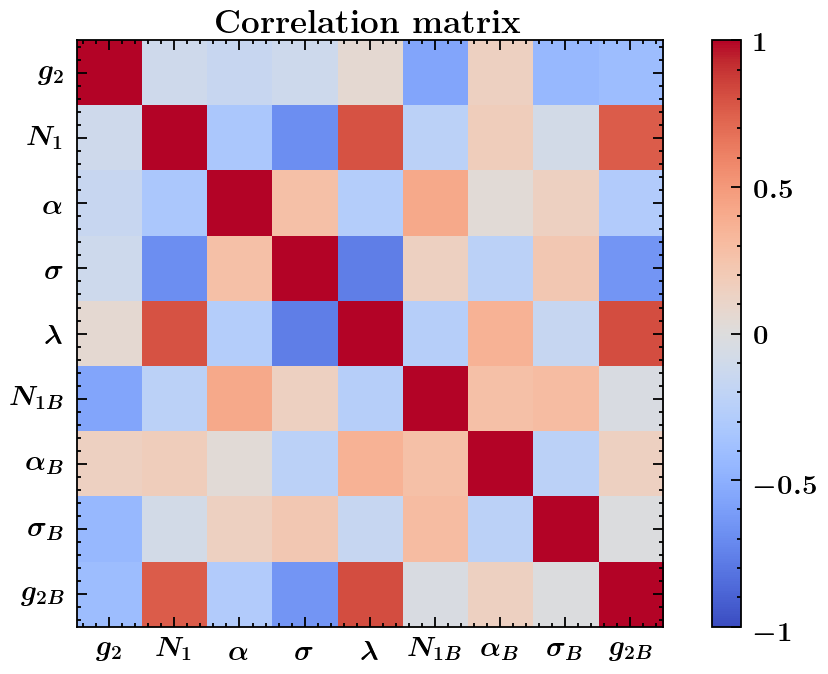
\includegraphics{pngplots/CorrelationMatrix.png}
\caption{Fitted parameter correlation matrix}
\end{figure}

\hypertarget{fit-properties}{%
\subsection{Fit properties}\label{fit-properties}}

\begin{figure}
\centering
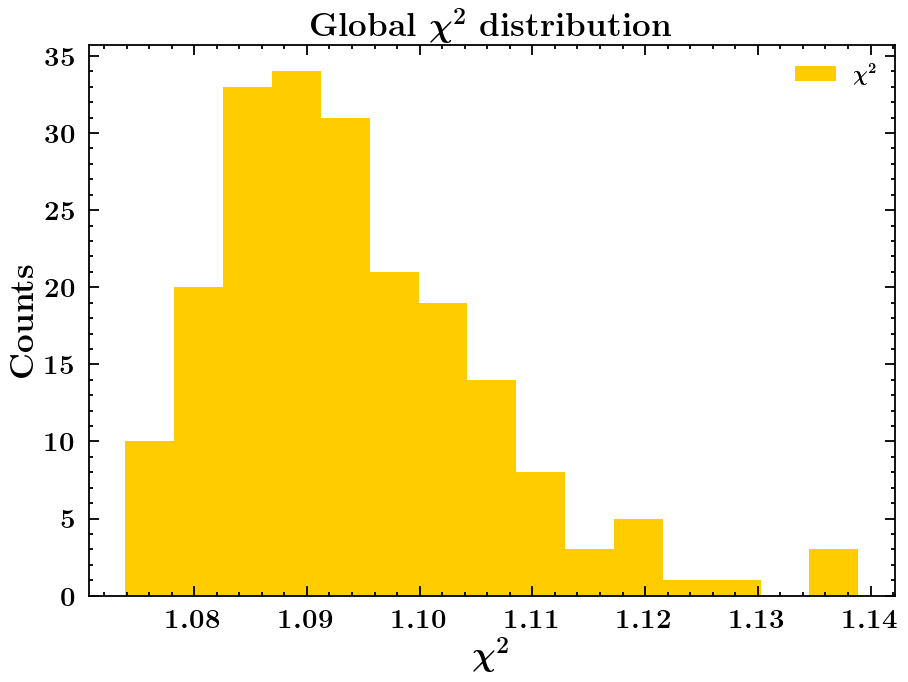
\includegraphics{pngplots/Globalchi2.png}
\caption{Global \(\chi^2\) distribution}
\end{figure}

\begin{figure}
\centering
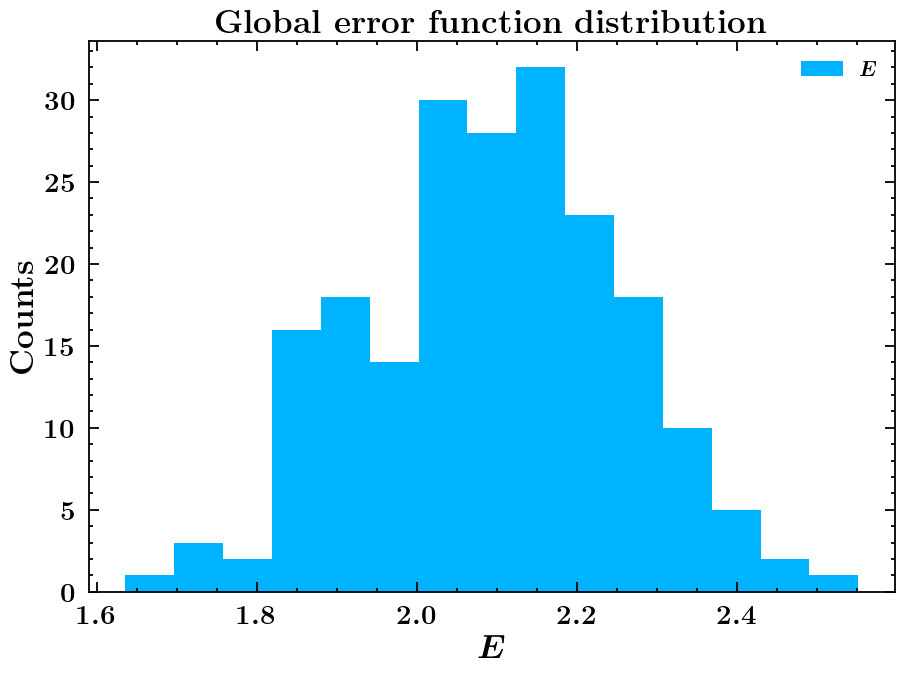
\includegraphics{pngplots/GlobalErrorFunction.png}
\caption{Global error function distribution}
\end{figure}

\begin{figure}
\centering
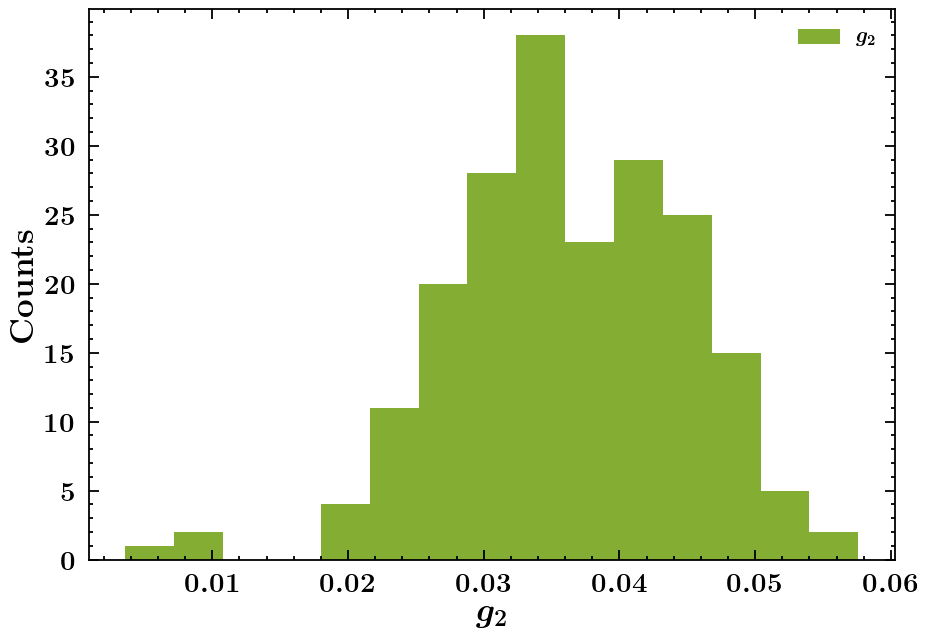
\includegraphics{pngplots/param0.png}
\caption{\(g_2\) distribution}
\end{figure}

\begin{figure}
\centering
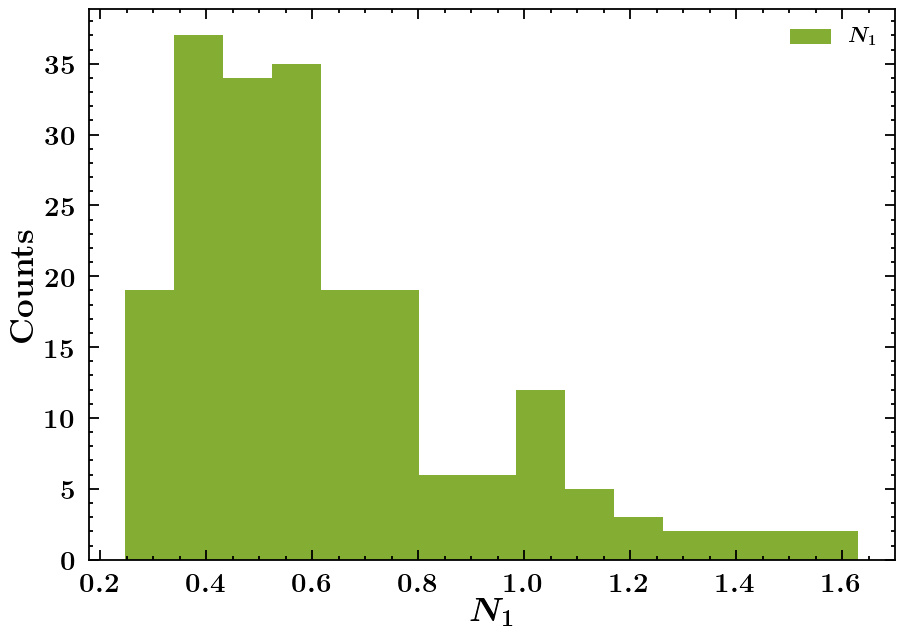
\includegraphics{pngplots/param1.png}
\caption{\(N_1\) distribution}
\end{figure}

\begin{figure}
\centering
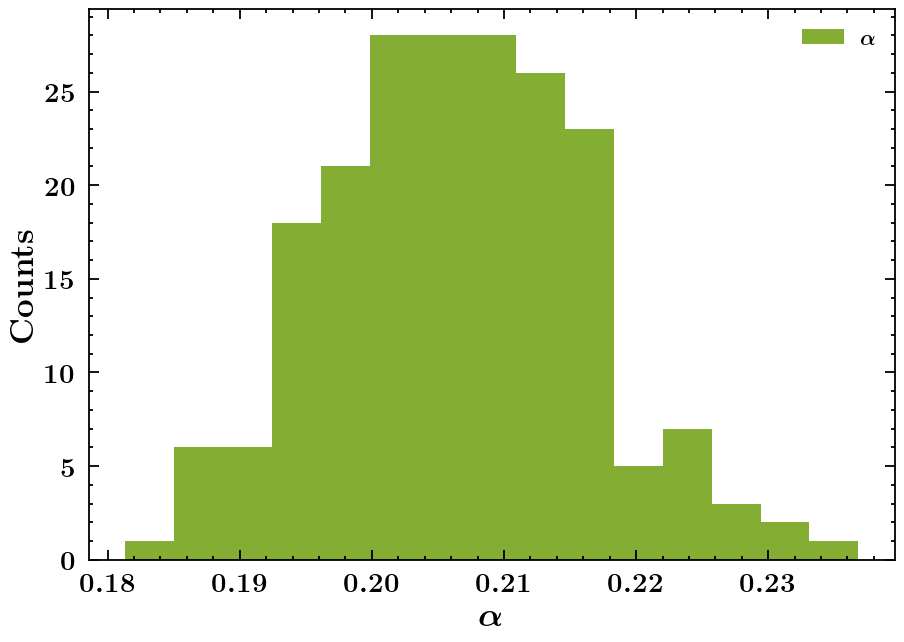
\includegraphics{pngplots/param2.png}
\caption{\(\alpha\) distribution}
\end{figure}

\begin{figure}
\centering
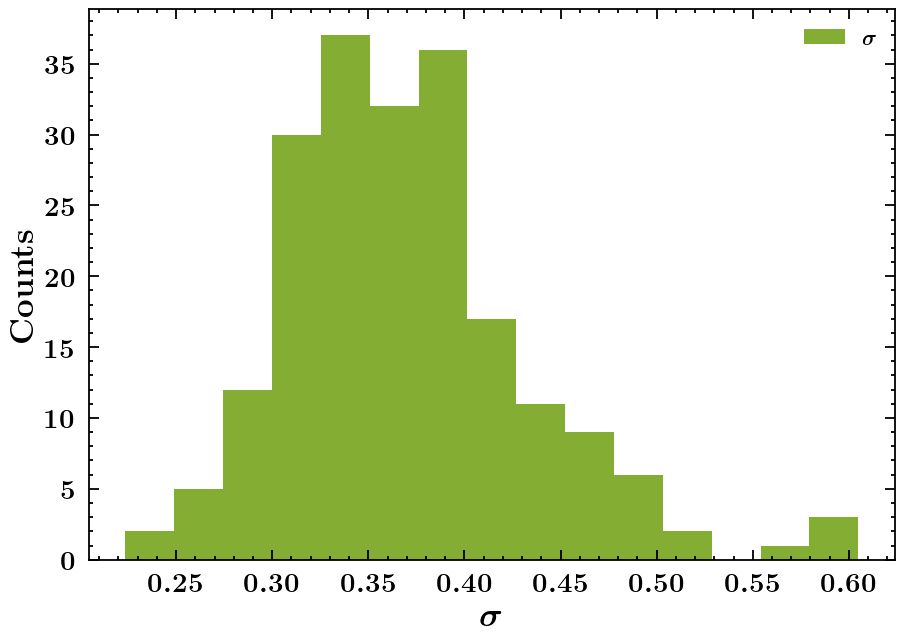
\includegraphics{pngplots/param3.png}
\caption{\(\sigma\) distribution}
\end{figure}

\begin{figure}
\centering
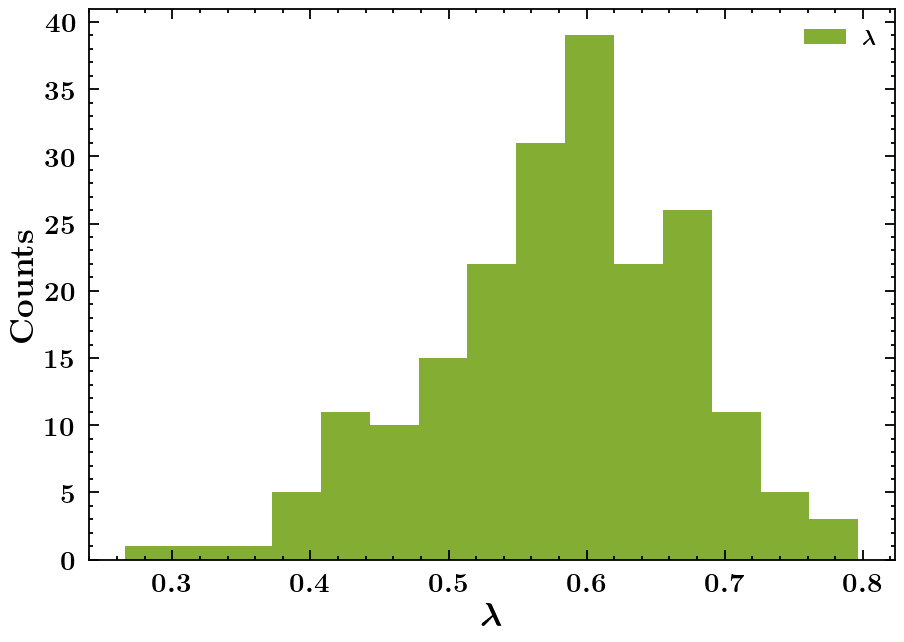
\includegraphics{pngplots/param4.png}
\caption{\(\lambda\) distribution}
\end{figure}

\begin{figure}
\centering
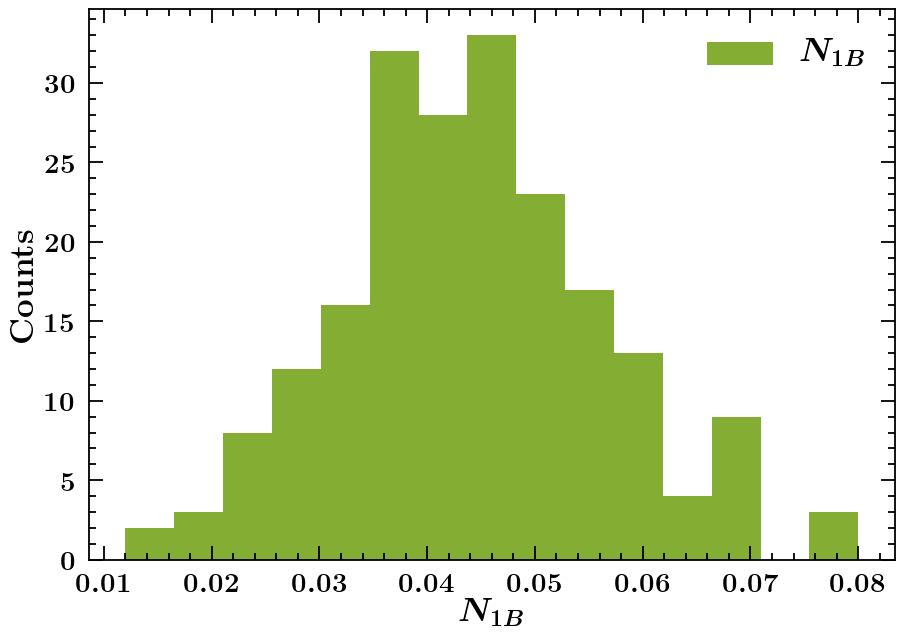
\includegraphics{pngplots/param5.png}
\caption{\(N_{1B}\) distribution}
\end{figure}

\begin{figure}
\centering
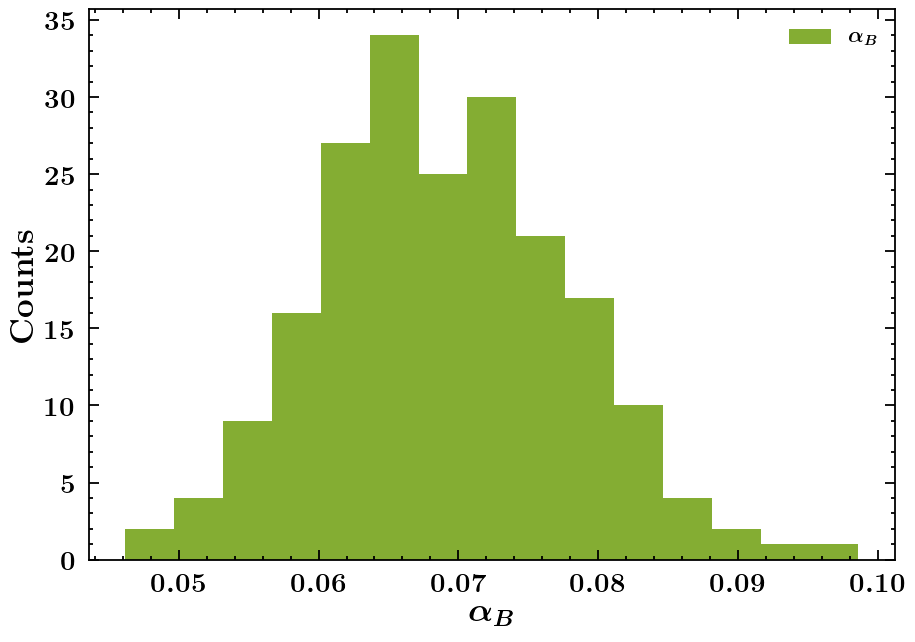
\includegraphics{pngplots/param6.png}
\caption{\(\alpha_B\) distribution}
\end{figure}

\begin{figure}
\centering
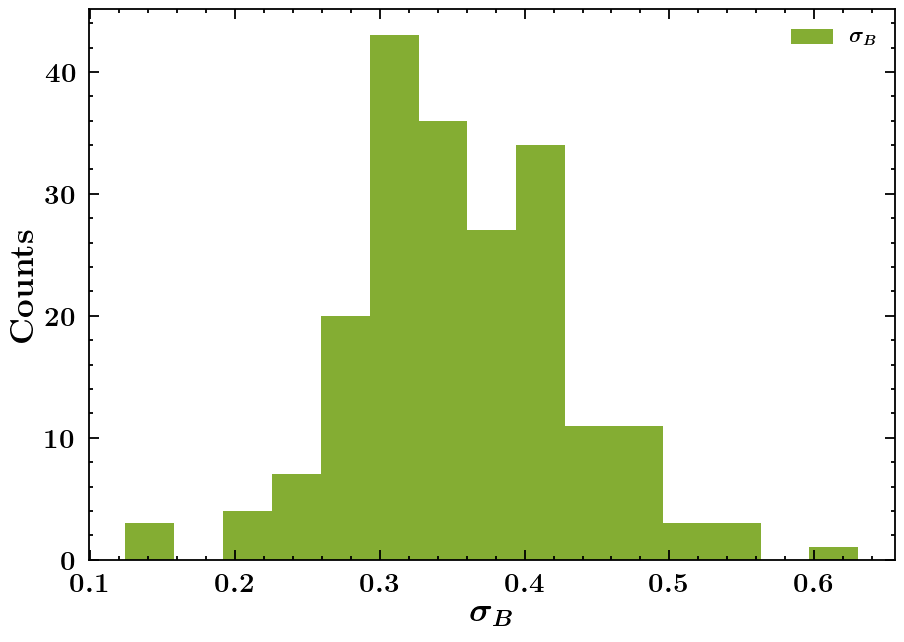
\includegraphics{pngplots/param7.png}
\caption{\(\sigma_B\) distribution}
\end{figure}

\begin{figure}
\centering
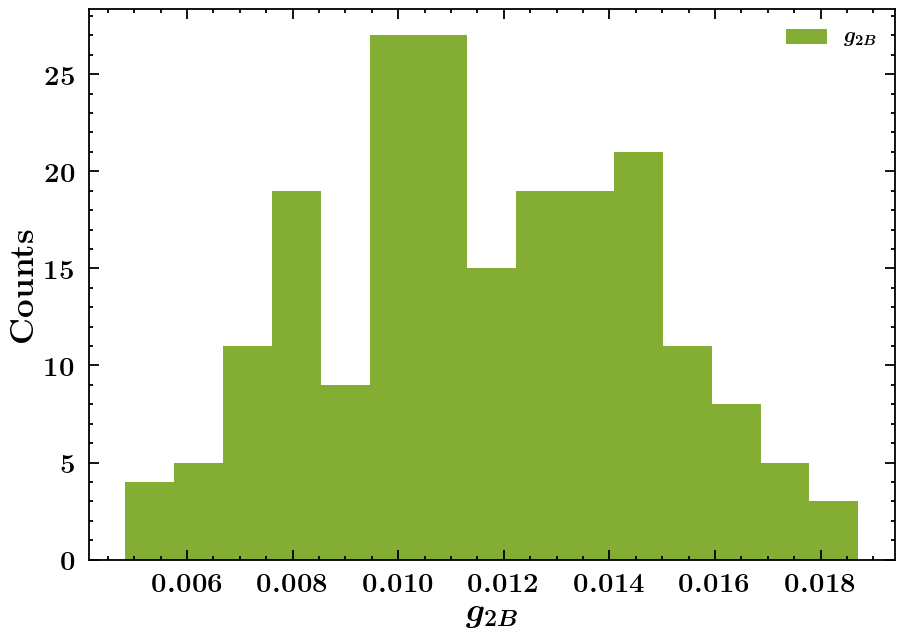
\includegraphics{pngplots/param8.png}
\caption{\(g_{2B}\) distribution}
\end{figure}

\hypertarget{table-of-chi2s}{%
\subsection{\texorpdfstring{Table of
\(\chi^2\)'s}{Table of \textbackslash chi\^{}2's}}\label{table-of-chi2s}}

\begin{table}[h]

\centering

\begin{tabular}{|c|c|c|c|c|} \hline

\textbf{Experiment} & \textbf{Number of
points} & \textbf{\(\chi_{D}^2\)} & \textbf{\(\chi_{\lambda}^2\)} & \textbf{\(\chi^2\)} \\ \hline

E605\_Q\_7\_8 & 7 & 0.669 & 0.0076 & 0.6766 \\ \hline
E605\_Q\_8\_9 & 8 & 1.5169 & 0.0046 & 1.5215 \\ \hline
E605\_Q\_10.5\_11.5 & 10 & 0.3414 & 0.1726 & 0.5139 \\ \hline
E605\_Q\_11.5\_13.5 & 12 & 0.7995 & 0.4912 & 1.2908 \\ \hline
E605\_Q\_13.5\_18 & 13 & 1.4071 & 0.6099 & 2.0171 \\ \hline
E288\_200\_Q\_4\_5 & 4 & 0.5246 & 0.8428 & 1.3674 \\ \hline
E288\_200\_Q\_5\_6 & 5 & 1.364 & 0.2684 & 1.6324 \\ \hline
E288\_200\_Q\_6\_7 & 6 & 0.2594 & 0.1346 & 0.3939 \\ \hline
E288\_200\_Q\_7\_8 & 7 & 0.4043 & 0.0047 & 0.409 \\ \hline
E288\_200\_Q\_8\_9 & 8 & 0.5483 & 0.044 & 0.5923 \\ \hline
E288\_300\_Q\_4\_5 & 4 & 0.4666 & 0.5624 & 1.0291 \\ \hline
E288\_300\_Q\_5\_6 & 5 & 0.7551 & 0.1563 & 0.9114 \\ \hline
E288\_300\_Q\_6\_7 & 6 & 0.4136 & 0.0334 & 0.447 \\ \hline
E288\_300\_Q\_7\_8 & 7 & 0.0881 & 0.0142 & 0.1023 \\ \hline
E288\_300\_Q\_8\_9 & 8 & 0.5524 & 0.0035 & 0.5559 \\ \hline
E288\_300\_Q\_11\_12 & 9 & 0.3573 & 0.2477 & 0.6051 \\ \hline
E288\_400\_Q\_5\_6 & 5 & 0.2659 & 0.0093 & 0.2752 \\ \hline
E288\_400\_Q\_6\_7 & 6 & 0.0789 & 0.0004 & 0.0793 \\ \hline
E288\_400\_Q\_7\_8 & 7 & 0.021 & 0.0216 & 0.0426 \\ \hline
E288\_400\_Q\_8\_9 & 8 & 0.4131 & 0.0486 & 0.4617 \\ \hline
E288\_400\_Q\_11\_12 & 11 & 0.5099 & 0.0534 & 0.5633 \\ \hline
E288\_400\_Q\_12\_13 & 12 & 0.4894 & 0.0484 & 0.5377 \\ \hline
E288\_400\_Q\_13\_14 & 12 & 0.5916 & 0.0931 & 0.6847 \\ \hline
STAR\_510 & 7 & 0.8905 & 0.0328 & 0.9233 \\ \hline
CDF\_RunI & 25 & 0.5329 & 0.0562 & 0.5891 \\ \hline
CDF\_RunII & 26 & 0.8728 & 0.0028 & 0.8756 \\ \hline
D0\_RunI & 12 & 0.6251 & 0.0461 & 0.6712 \\ \hline
D0\_RunII & 5 & 1.1341 & 0.605 & 1.7391 \\ \hline
D0\_RunIImu & 3 & 3.2816 & 0.0276 & 3.3093 \\ \hline
LHCb\_7TeV & 7 & 1.125 & 0.1572 & 1.2823 \\ \hline
LHCb\_8TeV & 7 & 0.5407 & 0.0839 & 0.6246 \\ \hline
LHCb\_13TeV & 7 & 0.7863 & 0.0219 & 0.8082 \\ \hline
CMS\_7TeV & 4 & 2.1253 & 0 & 2.1253 \\ \hline
CMS\_8TeV & 4 & 1.4284 & 0.0061 & 1.4346 \\ \hline
ATLAS\_7TeV\_y\_0\_1 & 6 & 2.6516 & 0.0299 & 2.6814 \\ \hline
ATLAS\_7TeV\_y\_1\_2 & 6 & 4.2049 & 1.034 & 5.239 \\ \hline
ATLAS\_7TeV\_y\_2\_2.4 & 6 & 3.5142 & 0.3819 & 3.8961 \\ \hline
ATLAS\_8TeV\_y\_0\_0.4 & 6 & 2.0046 & 0.3549 & 2.3594 \\ \hline
ATLAS\_8TeV\_y\_0.4\_0.8 & 6 & 2.2023 & 0.2704 & 2.4726 \\ \hline
ATLAS\_8TeV\_y\_0.8\_1.2 & 6 & 0.8917 & 0.0636 & 0.9553 \\ \hline
ATLAS\_8TeV\_y\_1.2\_1.6 & 6 & 0.9147 & 0.101 & 1.0157 \\ \hline
ATLAS\_8TeV\_y\_1.6\_2 & 6 & 0.611 & 0.0787 & 0.6897 \\ \hline
ATLAS\_8TeV\_y\_2\_2.4 & 6 & 0.7221 & 0.2993 & 1.0213 \\ \hline
ATLAS\_8TeV\_Q\_46\_66 & 4 & 2.3037 & 0.6971 & 3.0007 \\ \hline
ATLAS\_8TeV\_Q\_116\_150 & 8 & 0.4959 & 0.0029 & 0.4988 \\ \hline
Total & 353 & - & - & 1.0705 \\ \hline

\end{tabular}

\caption{Central-replica \(\chi^2\)'s:}

\end{table}

\begin{table}[h]

\centering

\begin{tabular}{|c|c|c|c|c|} \hline

\textbf{Experiment} & \textbf{Number of
points} & \textbf{\(\chi_{D}^2\)} & \textbf{\(\chi_{\lambda}^2\)} & \textbf{\(\chi^2\)} \\ \hline

E605\_Q\_7\_8 & 7 & 0.4192 & 0.0676 & 0.4868 \\ \hline
E605\_Q\_8\_9 & 8 & 0.9947 & 0.0338 & 1.0285 \\ \hline
E605\_Q\_10.5\_11.5 & 10 & 0.1911 & 0.1373 & 0.3284 \\ \hline
E605\_Q\_11.5\_13.5 & 12 & 0.4908 & 0.2839 & 0.7747 \\ \hline
E605\_Q\_13.5\_18 & 13 & 0.4912 & 0.3855 & 0.8767 \\ \hline
E288\_200\_Q\_4\_5 & 4 & 0.2132 & 0.6485 & 0.8617 \\ \hline
E288\_200\_Q\_5\_6 & 5 & 0.6733 & 0.2916 & 0.9649 \\ \hline
E288\_200\_Q\_6\_7 & 6 & 0.1334 & 0.1412 & 0.2746 \\ \hline
E288\_200\_Q\_7\_8 & 7 & 0.2543 & 0.0138 & 0.2681 \\ \hline
E288\_200\_Q\_8\_9 & 8 & 0.6522 & 0.0242 & 0.6764 \\ \hline
E288\_300\_Q\_4\_5 & 4 & 0.2307 & 0.5547 & 0.7854 \\ \hline
E288\_300\_Q\_5\_6 & 5 & 0.5024 & 0.2039 & 0.7063 \\ \hline
E288\_300\_Q\_6\_7 & 6 & 0.3153 & 0.0627 & 0.378 \\ \hline
E288\_300\_Q\_7\_8 & 7 & 0.0555 & 0.0301 & 0.0856 \\ \hline
E288\_300\_Q\_8\_9 & 8 & 0.5299 & 0.0169 & 0.5468 \\ \hline
E288\_300\_Q\_11\_12 & 9 & 1.0472 & 0.1675 & 1.2146 \\ \hline
E288\_400\_Q\_5\_6 & 5 & 0.3122 & 0.0652 & 0.3773 \\ \hline
E288\_400\_Q\_6\_7 & 6 & 0.0999 & 0.0046 & 0.1045 \\ \hline
E288\_400\_Q\_7\_8 & 7 & 0.0179 & 0.0112 & 0.0292 \\ \hline
E288\_400\_Q\_8\_9 & 8 & 0.4375 & 0.0392 & 0.4767 \\ \hline
E288\_400\_Q\_11\_12 & 11 & 0.6371 & 0.0362 & 0.6732 \\ \hline
E288\_400\_Q\_12\_13 & 12 & 0.7879 & 0.0279 & 0.8158 \\ \hline
E288\_400\_Q\_13\_14 & 12 & 1.0635 & 0.0436 & 1.1071 \\ \hline
STAR\_510 & 7 & 0.782 & 0.0538 & 0.8358 \\ \hline
CDF\_RunI & 25 & 0.4798 & 0.058 & 0.5377 \\ \hline
CDF\_RunII & 26 & 0.9586 & 0.0007 & 0.9593 \\ \hline
D0\_RunI & 12 & 0.7108 & 0.0426 & 0.7534 \\ \hline
D0\_RunII & 5 & 1.3252 & 0.6119 & 1.9371 \\ \hline
D0\_RunIImu & 3 & 3.1957 & 0.0226 & 3.2183 \\ \hline
LHCb\_7TeV & 7 & 1.0689 & 0.1942 & 1.263 \\ \hline
LHCb\_8TeV & 7 & 0.4598 & 0.0748 & 0.5346 \\ \hline
LHCb\_13TeV & 7 & 0.735 & 0.0199 & 0.7549 \\ \hline
CMS\_7TeV & 4 & 2.1314 & 0 & 2.1314 \\ \hline
CMS\_8TeV & 4 & 1.4053 & 0.0071 & 1.4124 \\ \hline
ATLAS\_7TeV\_y\_0\_1 & 6 & 2.5807 & 0.0281 & 2.6088 \\ \hline
ATLAS\_7TeV\_y\_1\_2 & 6 & 4.3332 & 1.0317 & 5.365 \\ \hline
ATLAS\_7TeV\_y\_2\_2.4 & 6 & 3.5606 & 0.3781 & 3.9386 \\ \hline
ATLAS\_8TeV\_y\_0\_0.4 & 6 & 1.9243 & 0.3374 & 2.2616 \\ \hline
ATLAS\_8TeV\_y\_0.4\_0.8 & 6 & 2.3423 & 0.2473 & 2.5896 \\ \hline
ATLAS\_8TeV\_y\_0.8\_1.2 & 6 & 0.917 & 0.0608 & 0.9778 \\ \hline
ATLAS\_8TeV\_y\_1.2\_1.6 & 6 & 0.9116 & 0.0945 & 1.0061 \\ \hline
ATLAS\_8TeV\_y\_1.6\_2 & 6 & 0.7211 & 0.0925 & 0.8136 \\ \hline
ATLAS\_8TeV\_y\_2\_2.4 & 6 & 0.9322 & 0.3482 & 1.2805 \\ \hline
ATLAS\_8TeV\_Q\_46\_66 & 4 & 2.1376 & 0.745 & 2.8826 \\ \hline
ATLAS\_8TeV\_Q\_116\_150 & 8 & 0.5006 & 0.0034 & 0.504 \\ \hline
Total & 353 & - & - & 1.0197 \\ \hline

\end{tabular}

\caption{Mean-replica \(\chi^2\)'s:}

\end{table}

\begin{table}[h]

\centering

\begin{tabular}{|c|c|c|} \hline

\textbf{Experiment} & \textbf{Number of
points} & \textbf{\(\chi^2\)} \\ \hline

E605\_Q\_7\_8 & 7 & 0.6923 \(\pm\) 0.1051 \\ \hline
E605\_Q\_8\_9 & 8 & 1.5366 \(\pm\) 0.2235 \\ \hline
E605\_Q\_10.5\_11.5 & 10 & 0.5526 \(\pm\) 0.0707 \\ \hline
E605\_Q\_11.5\_13.5 & 12 & 1.3868 \(\pm\) 0.1114 \\ \hline
E605\_Q\_13.5\_18 & 13 & 2.0448 \(\pm\) 0.1111 \\ \hline
E288\_200\_Q\_4\_5 & 4 & 1.4317 \(\pm\) 0.2871 \\ \hline
E288\_200\_Q\_5\_6 & 5 & 1.6681 \(\pm\) 0.1951 \\ \hline
E288\_200\_Q\_6\_7 & 6 & 0.4153 \(\pm\) 0.0841 \\ \hline
E288\_200\_Q\_7\_8 & 7 & 0.4252 \(\pm\) 0.1424 \\ \hline
E288\_200\_Q\_8\_9 & 8 & 0.6013 \(\pm\) 0.0674 \\ \hline
E288\_300\_Q\_4\_5 & 4 & 1.0873 \(\pm\) 0.2658 \\ \hline
E288\_300\_Q\_5\_6 & 5 & 0.9425 \(\pm\) 0.1367 \\ \hline
E288\_300\_Q\_6\_7 & 6 & 0.4611 \(\pm\) 0.1291 \\ \hline
E288\_300\_Q\_7\_8 & 7 & 0.1152 \(\pm\) 0.0447 \\ \hline
E288\_300\_Q\_8\_9 & 8 & 0.5761 \(\pm\) 0.1005 \\ \hline
E288\_300\_Q\_11\_12 & 9 & 0.6082 \(\pm\) 0.0286 \\ \hline
E288\_400\_Q\_5\_6 & 5 & 0.3165 \(\pm\) 0.0805 \\ \hline
E288\_400\_Q\_6\_7 & 6 & 0.1108 \(\pm\) 0.0304 \\ \hline
E288\_400\_Q\_7\_8 & 7 & 0.0818 \(\pm\) 0.0537 \\ \hline
E288\_400\_Q\_8\_9 & 8 & 0.5044 \(\pm\) 0.082 \\ \hline
E288\_400\_Q\_11\_12 & 11 & 0.595 \(\pm\) 0.1376 \\ \hline
E288\_400\_Q\_12\_13 & 12 & 0.5698 \(\pm\) 0.0392 \\ \hline
E288\_400\_Q\_13\_14 & 12 & 0.6966 \(\pm\) 0.0513 \\ \hline
STAR\_510 & 7 & 0.9304 \(\pm\) 0.0466 \\ \hline
CDF\_RunI & 25 & 0.5917 \(\pm\) 0.0158 \\ \hline
CDF\_RunII & 26 & 0.8965 \(\pm\) 0.066 \\ \hline
D0\_RunI & 12 & 0.6707 \(\pm\) 0.028 \\ \hline
D0\_RunII & 5 & 1.7018 \(\pm\) 0.2229 \\ \hline
D0\_RunIImu & 3 & 3.2127 \(\pm\) 0.4425 \\ \hline
LHCb\_7TeV & 7 & 1.2814 \(\pm\) 0.0368 \\ \hline
LHCb\_8TeV & 7 & 0.6692 \(\pm\) 0.1276 \\ \hline
LHCb\_13TeV & 7 & 0.8452 \(\pm\) 0.0693 \\ \hline
CMS\_7TeV & 4 & 2.128 \(\pm\) 0.0091 \\ \hline
CMS\_8TeV & 4 & 1.4324 \(\pm\) 0.0513 \\ \hline
ATLAS\_7TeV\_y\_0\_1 & 6 & 2.707 \(\pm\) 0.2419 \\ \hline
ATLAS\_7TeV\_y\_1\_2 & 6 & 5.2871 \(\pm\) 0.0938 \\ \hline
ATLAS\_7TeV\_y\_2\_2.4 & 6 & 3.9159 \(\pm\) 0.1081 \\ \hline
ATLAS\_8TeV\_y\_0\_0.4 & 6 & 2.3637 \(\pm\) 0.1339 \\ \hline
ATLAS\_8TeV\_y\_0.4\_0.8 & 6 & 2.5022 \(\pm\) 0.0868 \\ \hline
ATLAS\_8TeV\_y\_0.8\_1.2 & 6 & 0.9942 \(\pm\) 0.0849 \\ \hline
ATLAS\_8TeV\_y\_1.2\_1.6 & 6 & 1.0378 \(\pm\) 0.1538 \\ \hline
ATLAS\_8TeV\_y\_1.6\_2 & 6 & 0.8048 \(\pm\) 0.2414 \\ \hline
ATLAS\_8TeV\_y\_2\_2.4 & 6 & 1.0539 \(\pm\) 0.2233 \\ \hline
ATLAS\_8TeV\_Q\_46\_66 & 4 & 2.9948 \(\pm\) 0.1166 \\ \hline
ATLAS\_8TeV\_Q\_116\_150 & 8 & 0.5023 \(\pm\) 0.0081 \\ \hline
Total & 353 & 1.094 \(\pm\) 0.0119 \\ \hline

\end{tabular}

\caption{Average-over-replicas \(\chi^2\)'s:}

\end{table}

\hypertarget{tmds-in-k_t-space}{%
\subsection{\texorpdfstring{TMDs in \(k_T\)
space}{TMDs in k\_T space}}\label{tmds-in-k_t-space}}

\begin{figure}
\centering
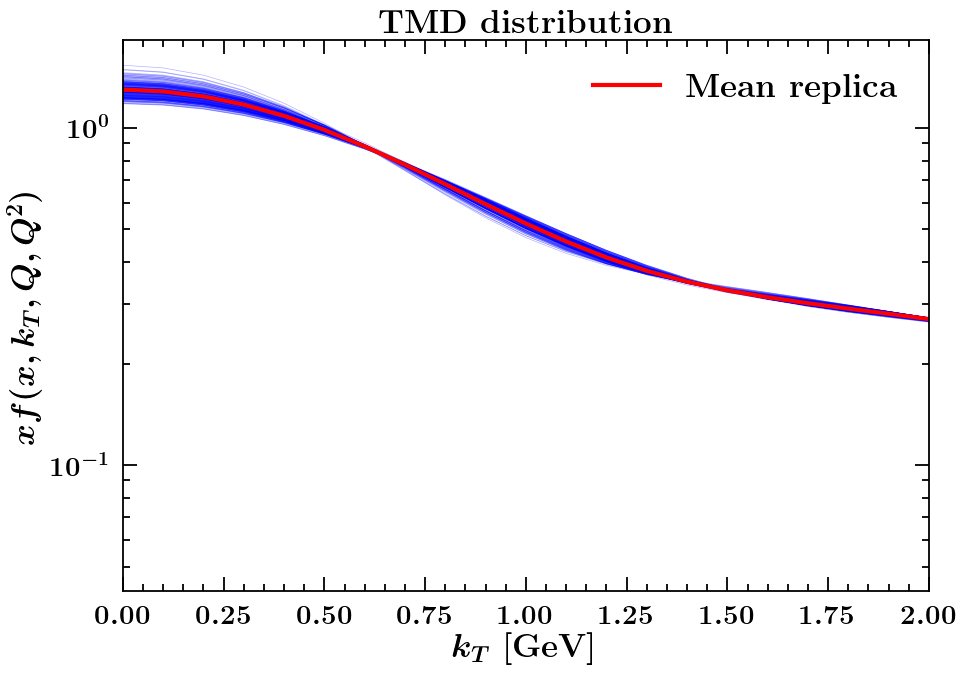
\includegraphics{pngplots/tmd_1_2_0.001.png}
\caption{TMD PDF of the \(d\) at \(Q = 2\) GeV and \(x = 0.001\)}
\end{figure}

\begin{figure}
\centering
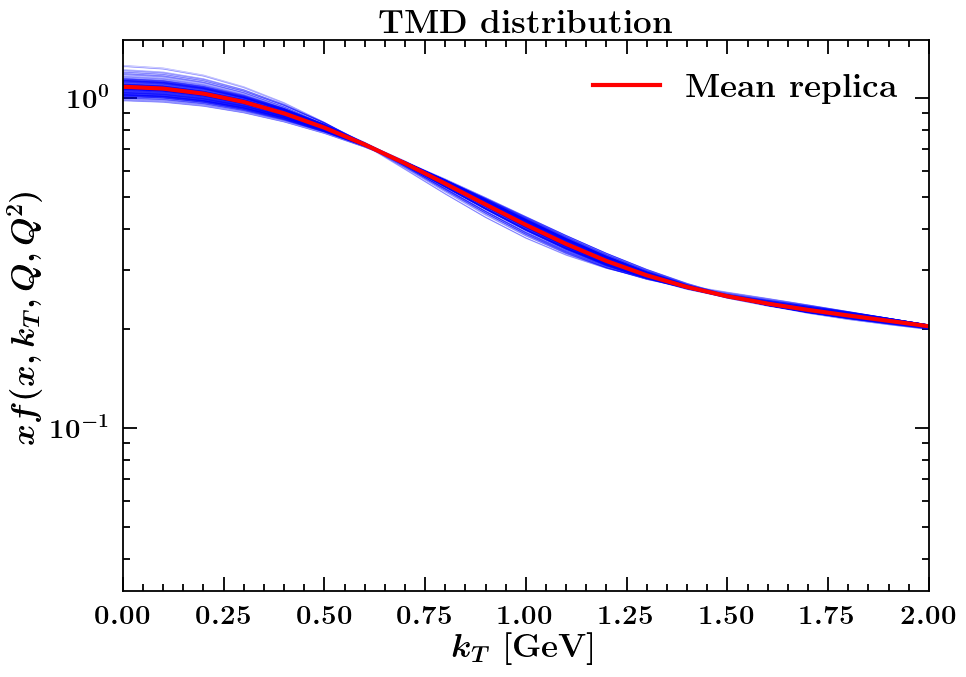
\includegraphics{pngplots/tmd_1_2_0.01.png}
\caption{TMD PDF of the \(d\) at \(Q = 2\) GeV and \(x = 0.01\)}
\end{figure}

\begin{figure}
\centering
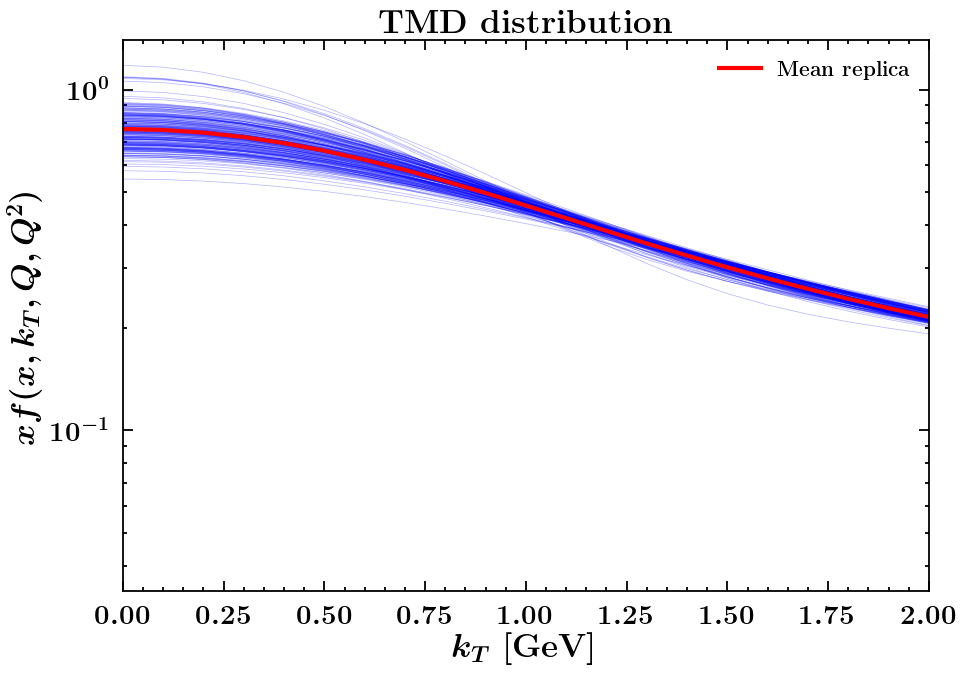
\includegraphics{pngplots/tmd_1_2_0.1.png}
\caption{TMD PDF of the \(d\) at \(Q = 2\) GeV and \(x = 0.1\)}
\end{figure}

\begin{figure}
\centering
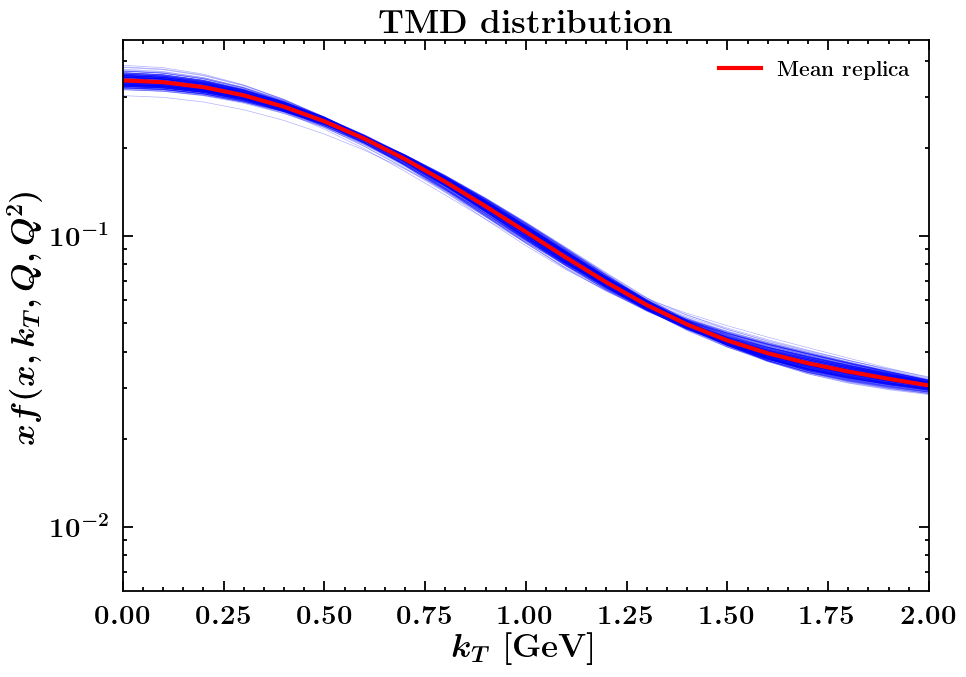
\includegraphics{pngplots/tmd_1_2_0.5.png}
\caption{TMD PDF of the \(d\) at \(Q = 2\) GeV and \(x = 0.5\)}
\end{figure}

\begin{figure}
\centering
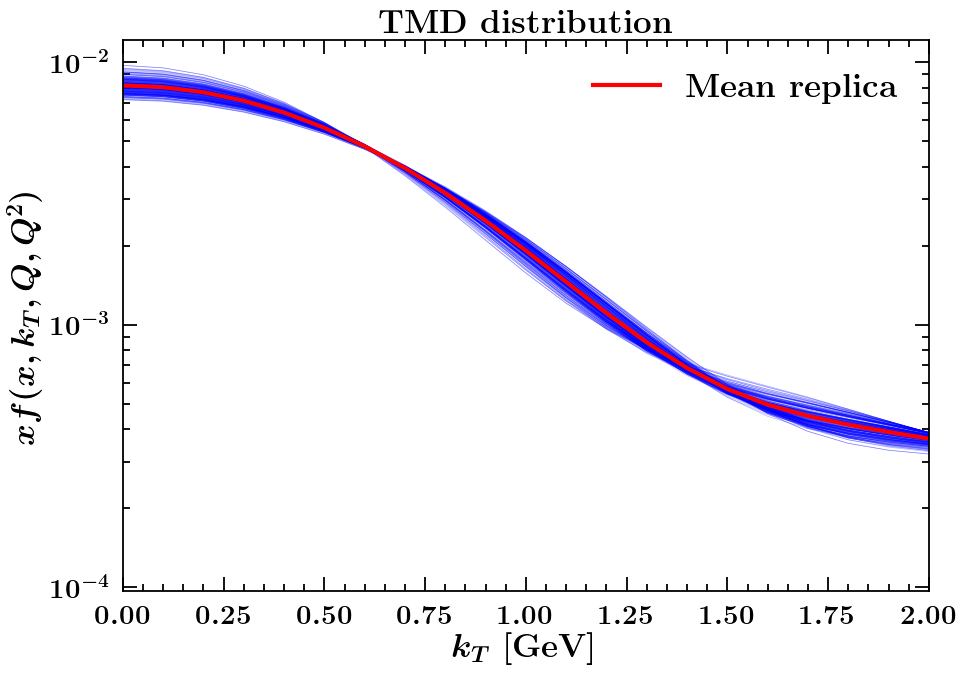
\includegraphics{pngplots/tmd_1_2_0.9.png}
\caption{TMD PDF of the \(d\) at \(Q = 2\) GeV and \(x = 0.9\)}
\end{figure}

\hypertarget{data-theory-comparison}{%
\subsection{Data-theory comparison}\label{data-theory-comparison}}

\begin{figure}
\centering
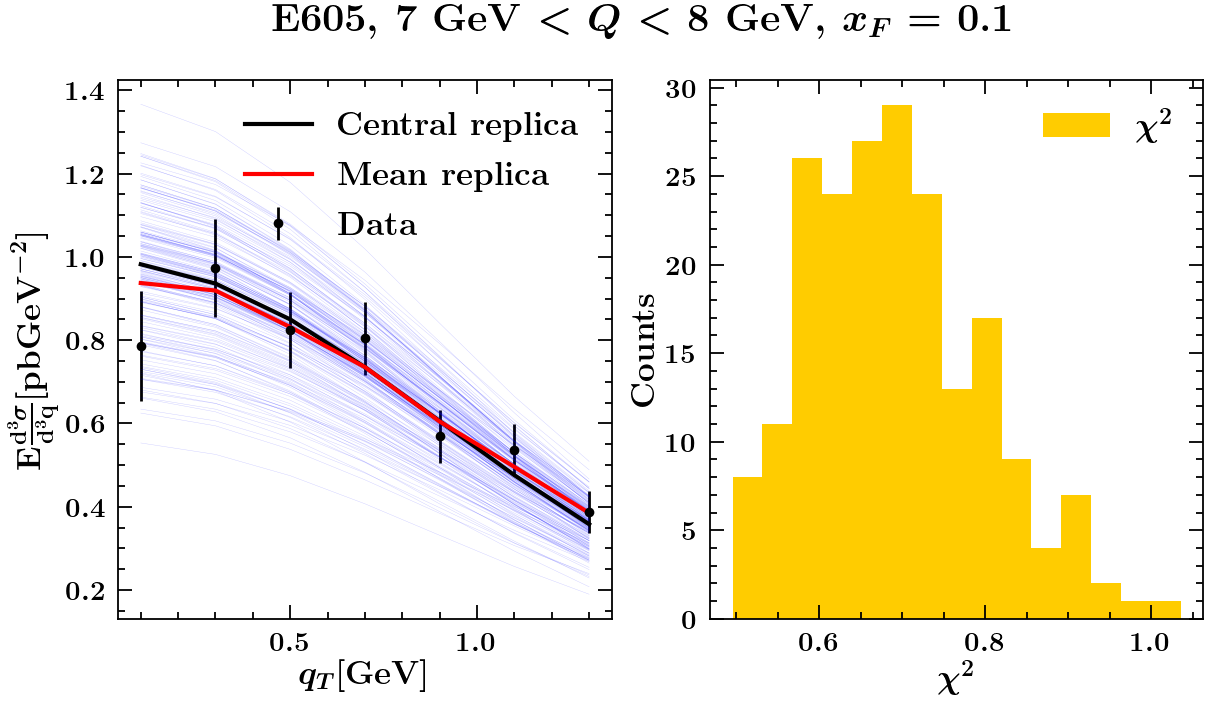
\includegraphics{pngplots/E605_Q_7_8.png}
\caption{E605\_Q\_7\_8 data-theory comparison}
\end{figure}

\begin{figure}
\centering
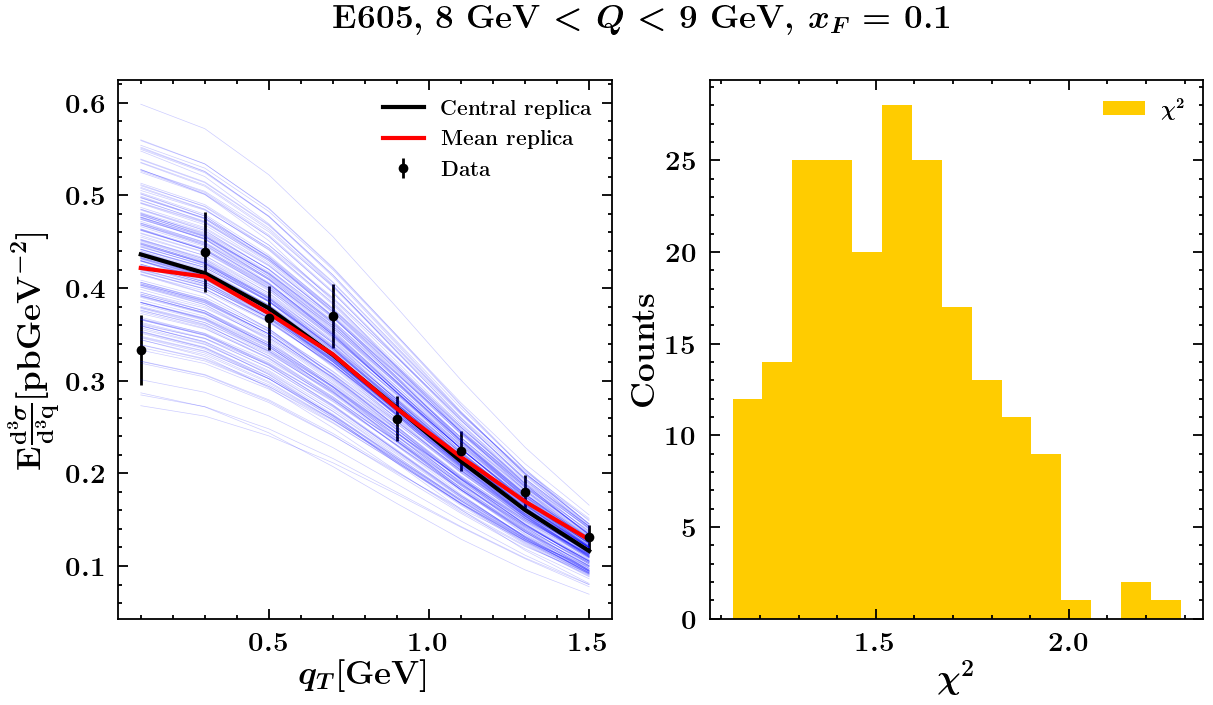
\includegraphics{pngplots/E605_Q_8_9.png}
\caption{E605\_Q\_8\_9 data-theory comparison}
\end{figure}

\begin{figure}
\centering
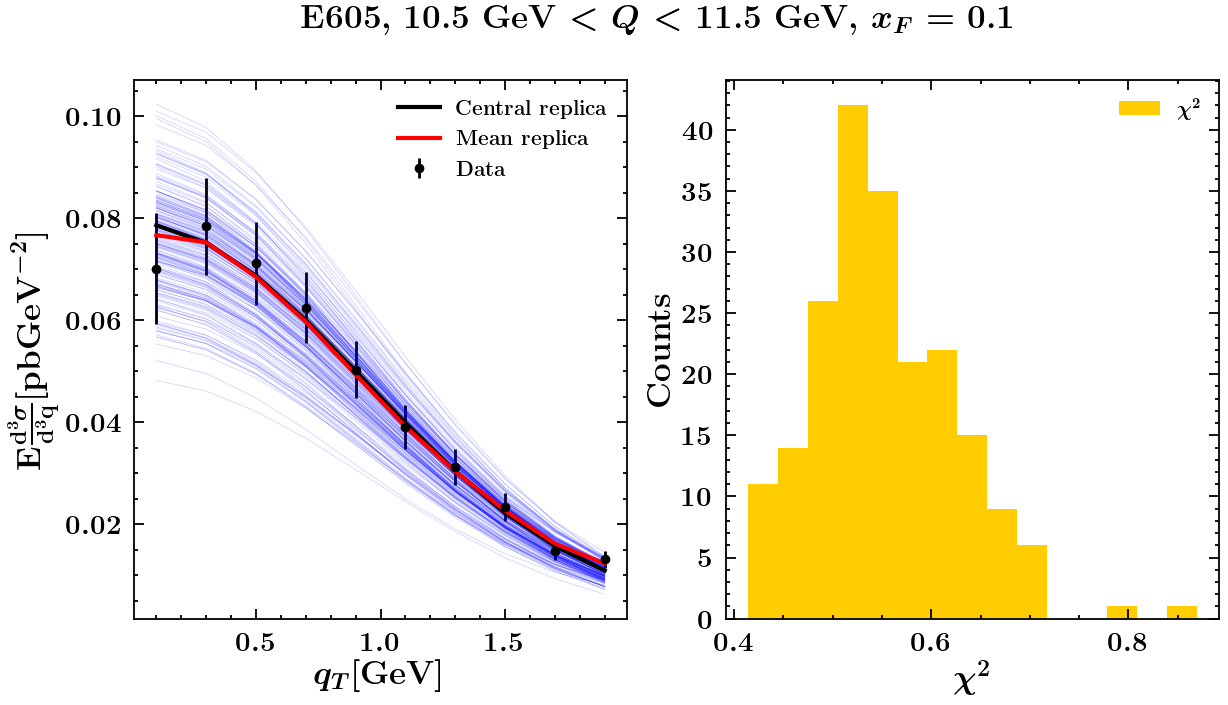
\includegraphics{pngplots/E605_Q_10.5_11.5.png}
\caption{E605\_Q\_10.5\_11.5 data-theory comparison}
\end{figure}

\begin{figure}
\centering
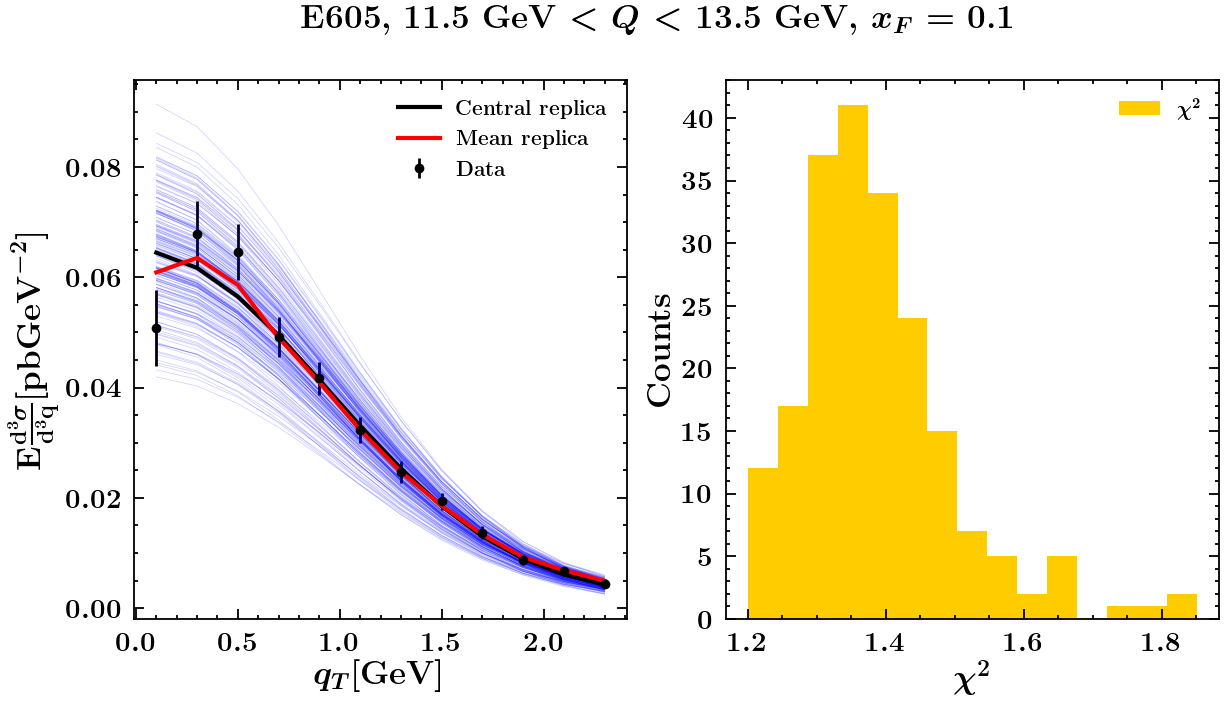
\includegraphics{pngplots/E605_Q_11.5_13.5.png}
\caption{E605\_Q\_11.5\_13.5 data-theory comparison}
\end{figure}

\begin{figure}
\centering
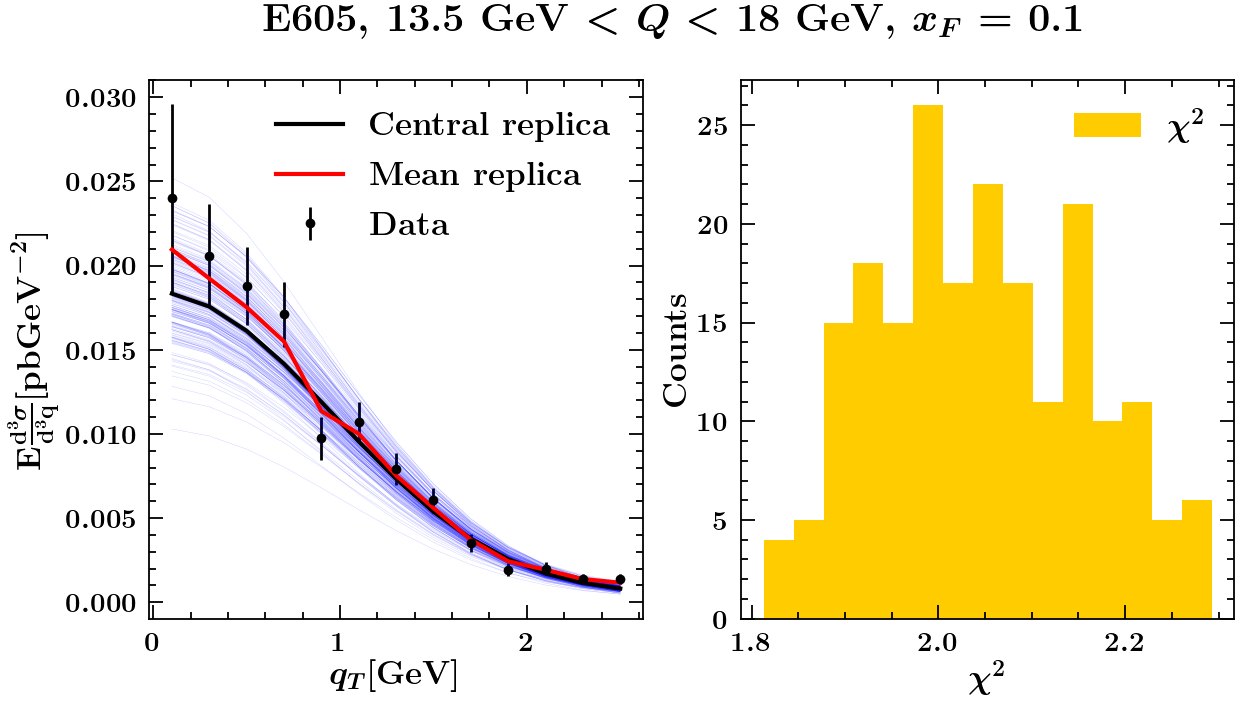
\includegraphics{pngplots/E605_Q_13.5_18.png}
\caption{E605\_Q\_13.5\_18 data-theory comparison}
\end{figure}

\begin{figure}
\centering
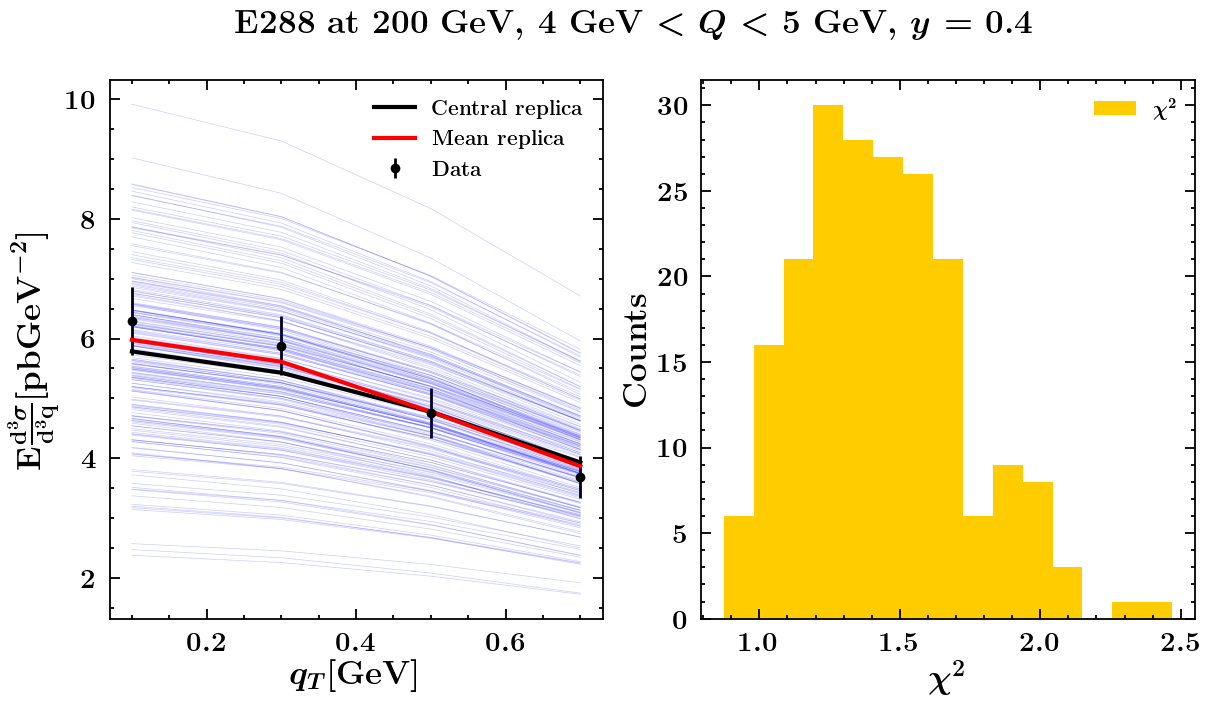
\includegraphics{pngplots/E288_200_Q_4_5.png}
\caption{E288\_200\_Q\_4\_5 data-theory comparison}
\end{figure}

\begin{figure}
\centering
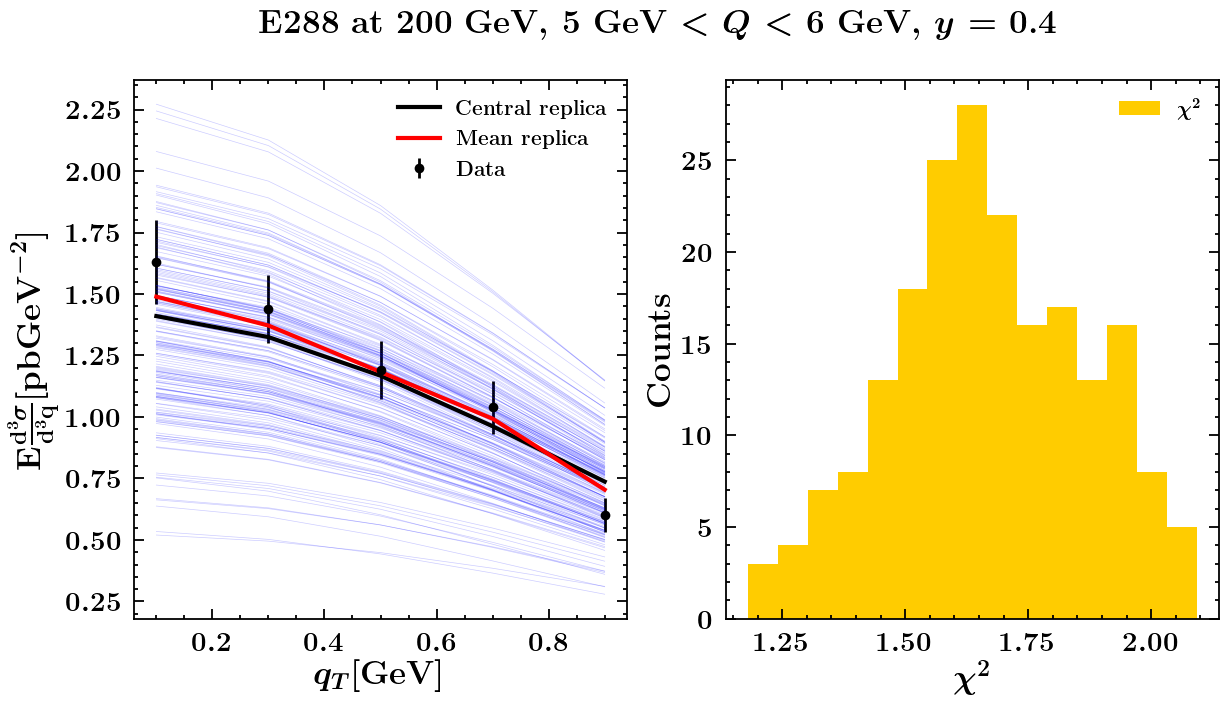
\includegraphics{pngplots/E288_200_Q_5_6.png}
\caption{E288\_200\_Q\_5\_6 data-theory comparison}
\end{figure}

\begin{figure}
\centering
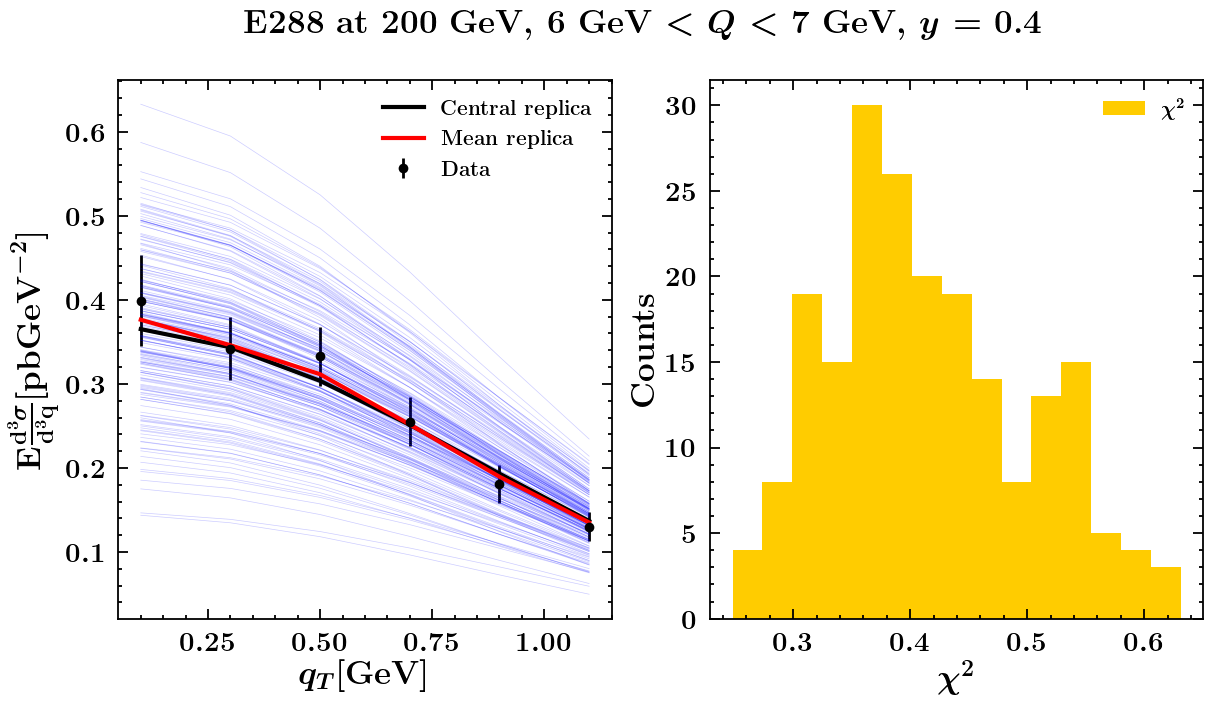
\includegraphics{pngplots/E288_200_Q_6_7.png}
\caption{E288\_200\_Q\_6\_7 data-theory comparison}
\end{figure}

\begin{figure}
\centering
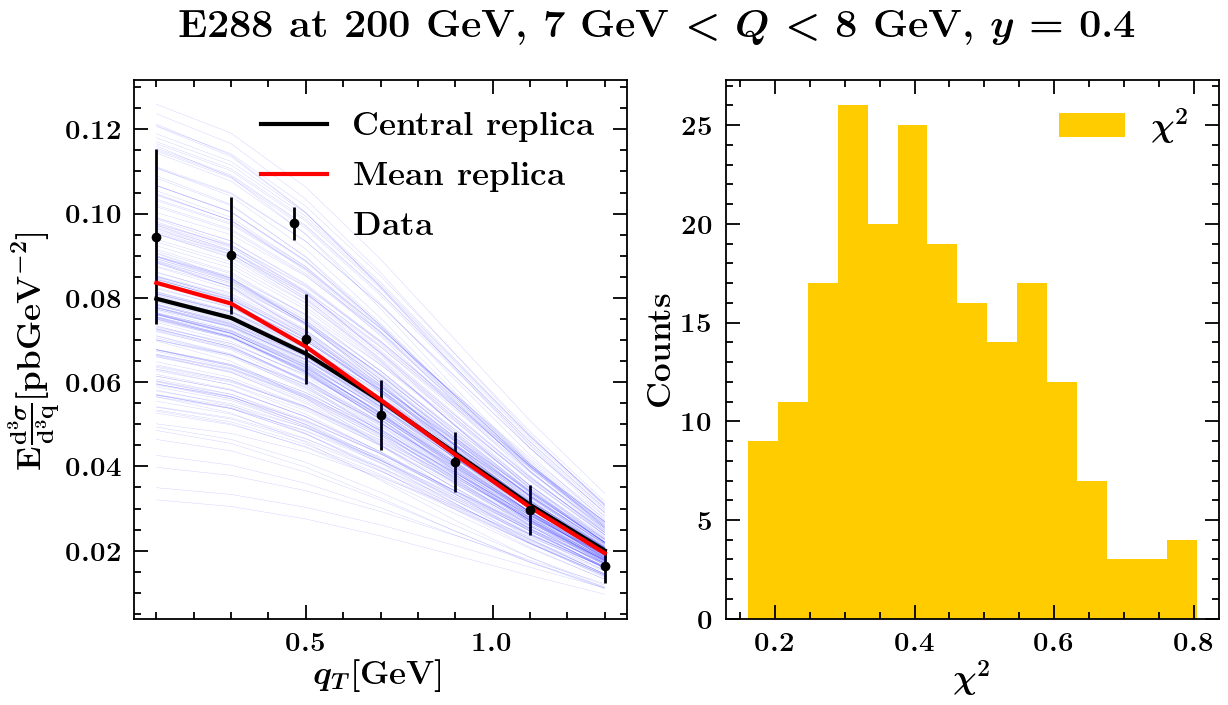
\includegraphics{pngplots/E288_200_Q_7_8.png}
\caption{E288\_200\_Q\_7\_8 data-theory comparison}
\end{figure}

\begin{figure}
\centering
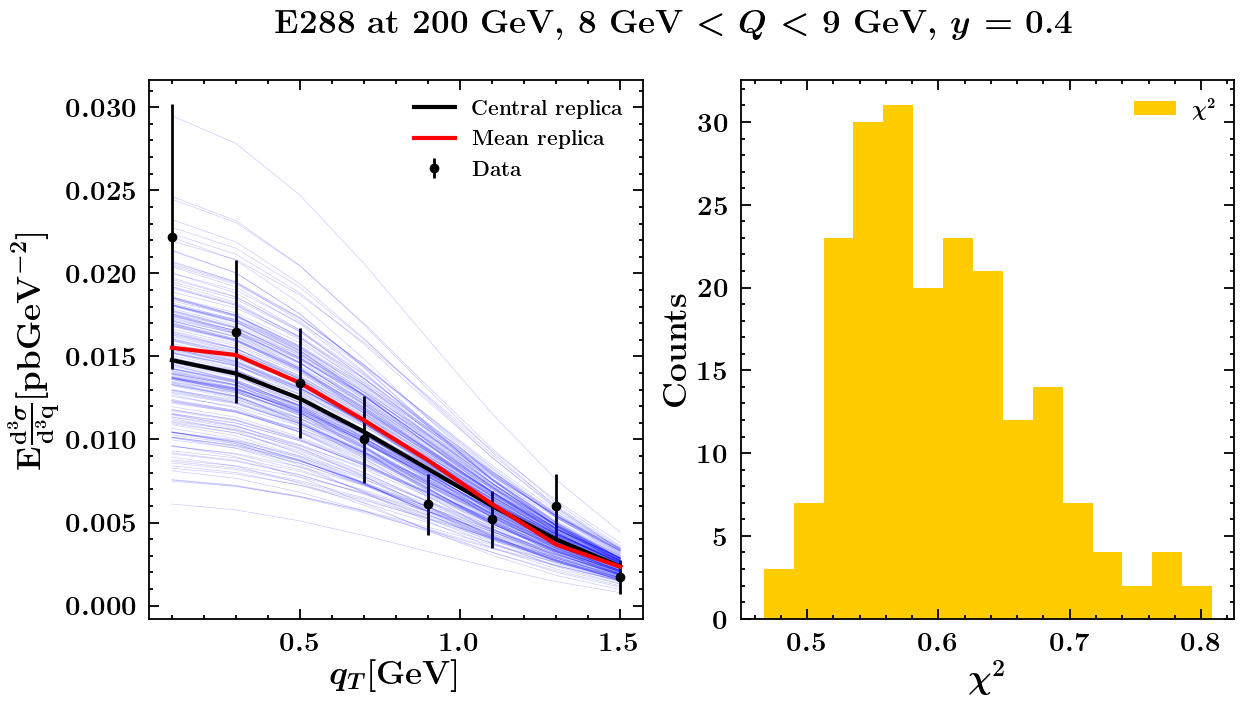
\includegraphics{pngplots/E288_200_Q_8_9.png}
\caption{E288\_200\_Q\_8\_9 data-theory comparison}
\end{figure}

\begin{figure}
\centering
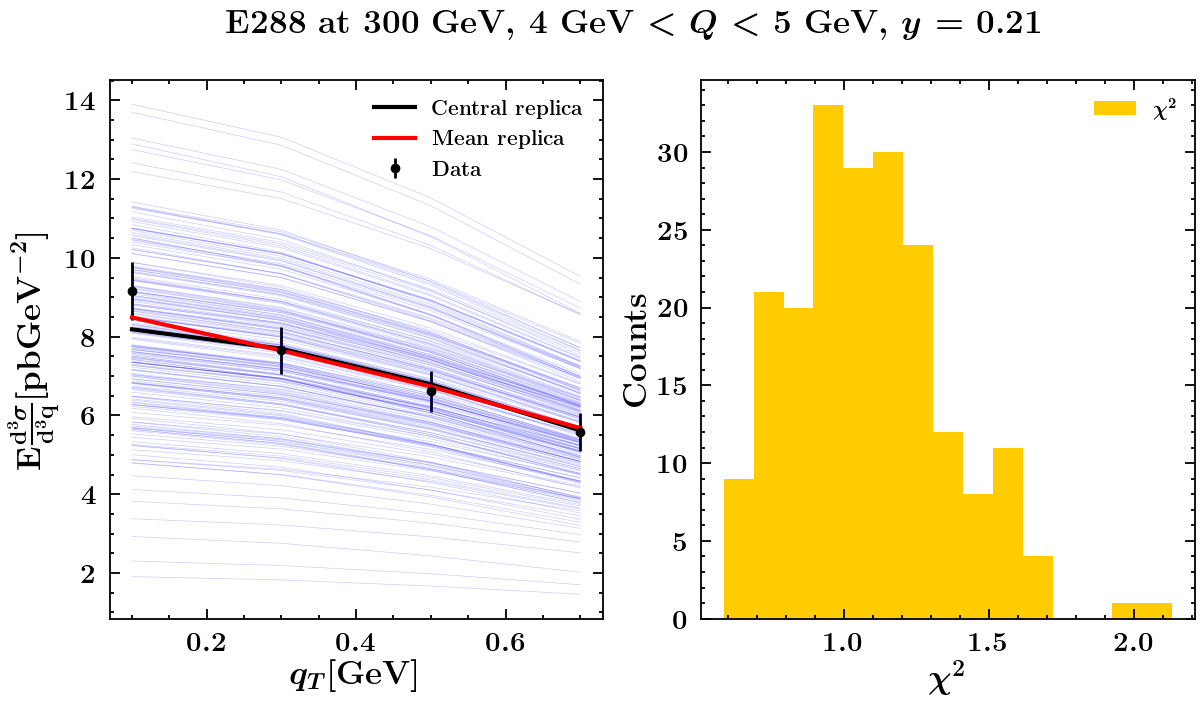
\includegraphics{pngplots/E288_300_Q_4_5.png}
\caption{E288\_300\_Q\_4\_5 data-theory comparison}
\end{figure}

\begin{figure}
\centering
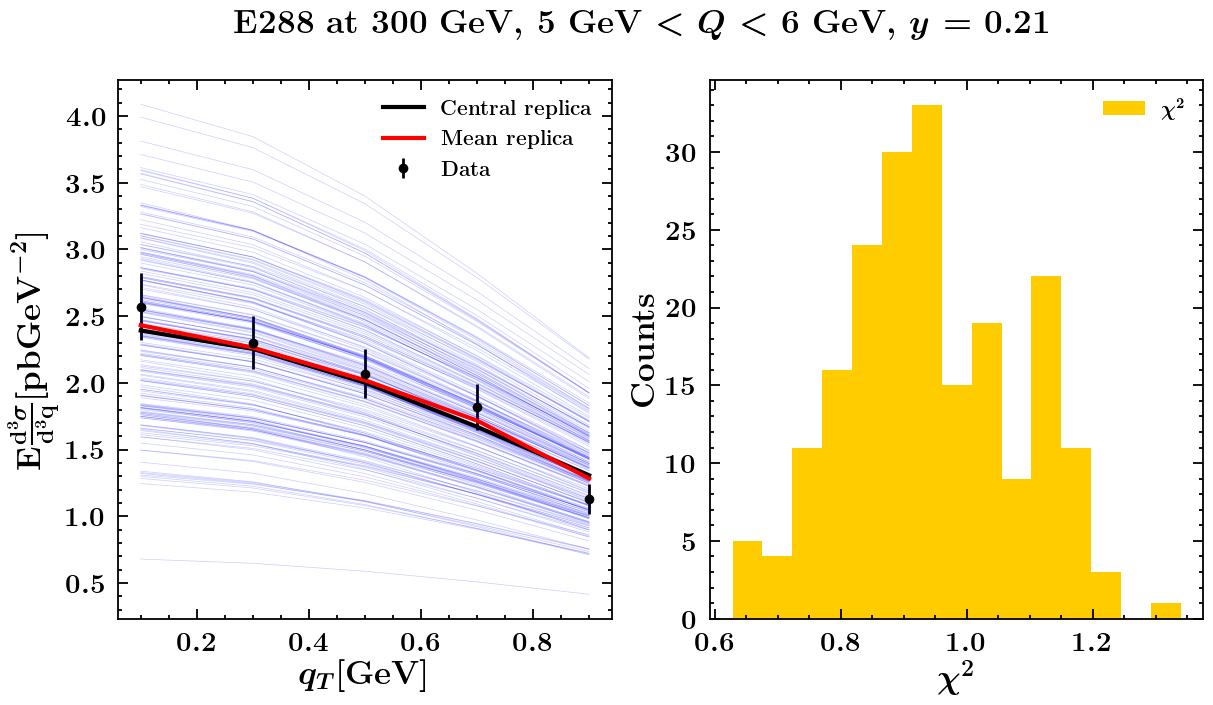
\includegraphics{pngplots/E288_300_Q_5_6.png}
\caption{E288\_300\_Q\_5\_6 data-theory comparison}
\end{figure}

\begin{figure}
\centering
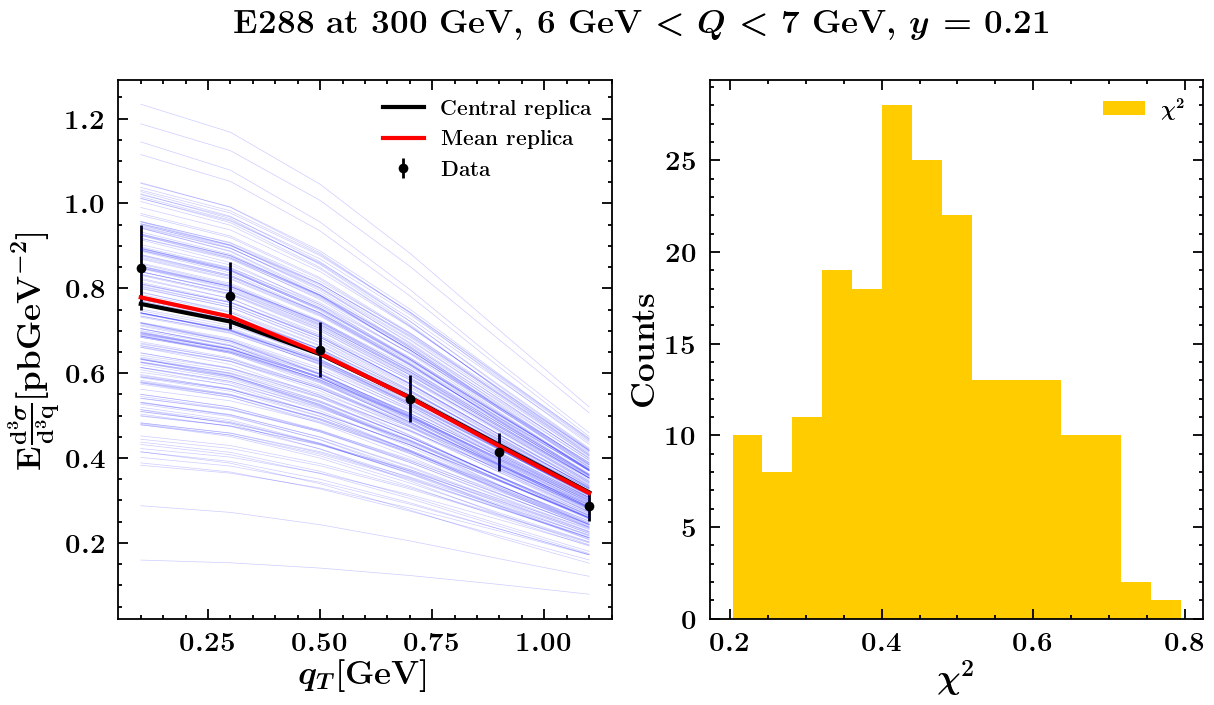
\includegraphics{pngplots/E288_300_Q_6_7.png}
\caption{E288\_300\_Q\_6\_7 data-theory comparison}
\end{figure}

\begin{figure}
\centering
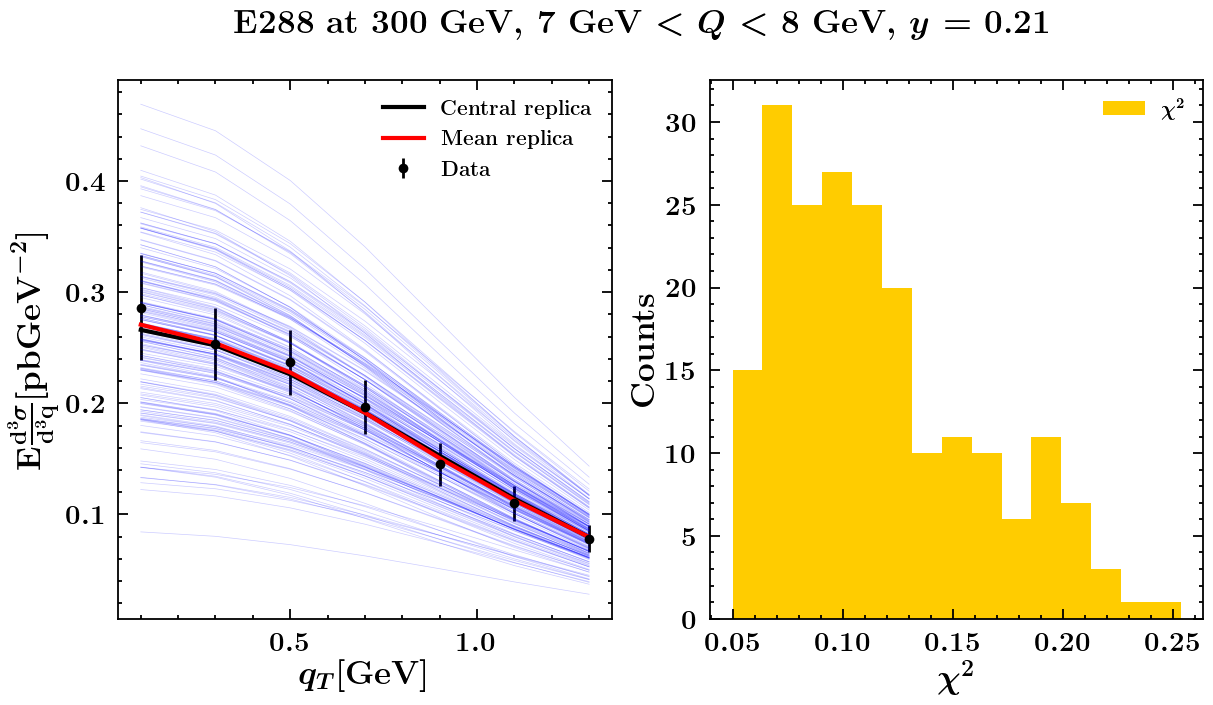
\includegraphics{pngplots/E288_300_Q_7_8.png}
\caption{E288\_300\_Q\_7\_8 data-theory comparison}
\end{figure}

\begin{figure}
\centering
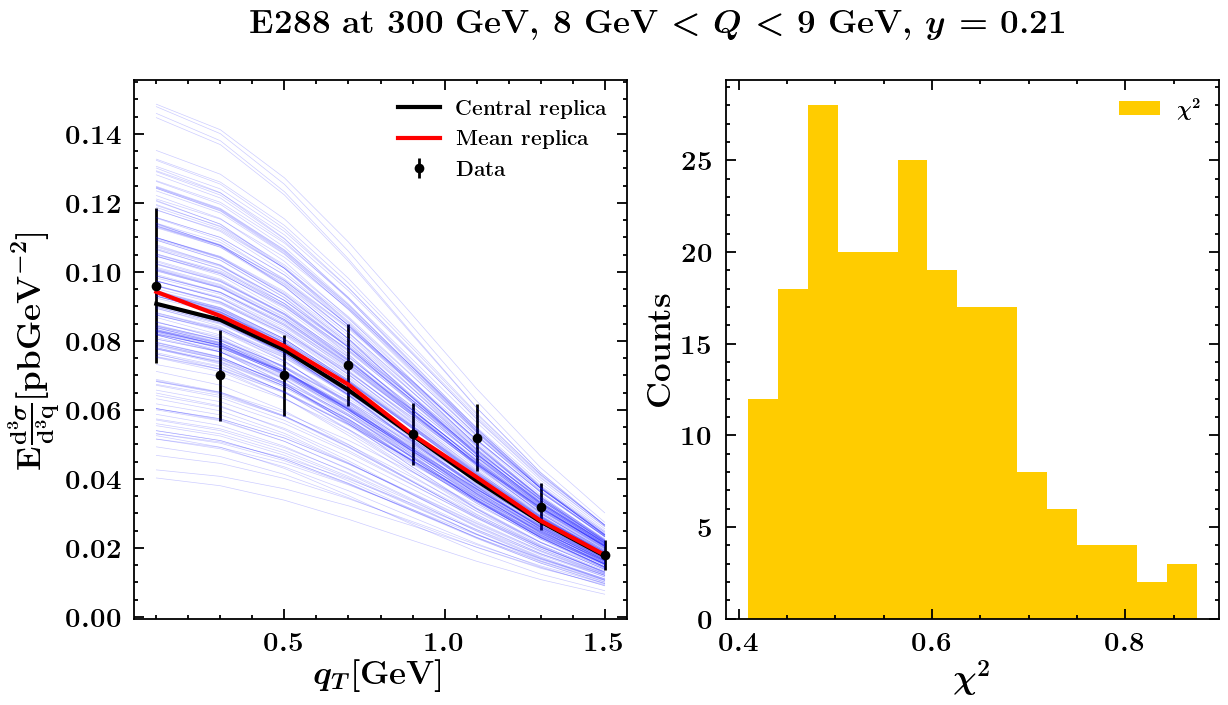
\includegraphics{pngplots/E288_300_Q_8_9.png}
\caption{E288\_300\_Q\_8\_9 data-theory comparison}
\end{figure}

\begin{figure}
\centering
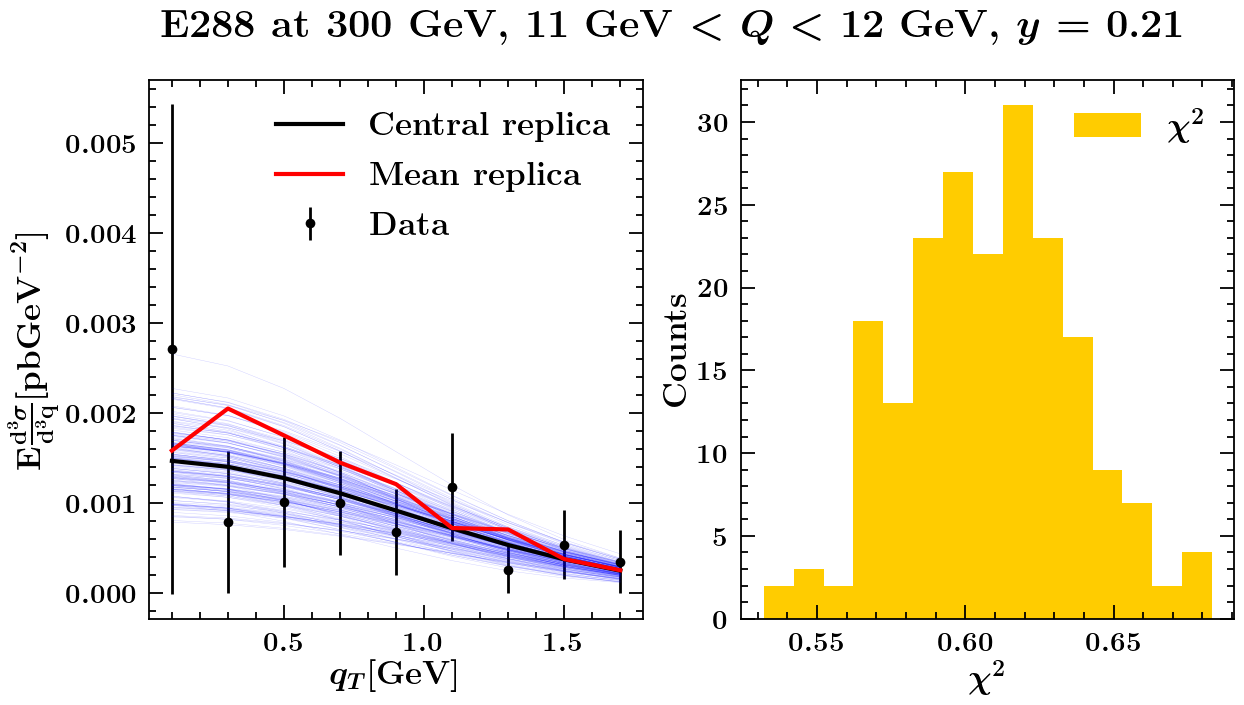
\includegraphics{pngplots/E288_300_Q_11_12.png}
\caption{E288\_300\_Q\_11\_12 data-theory comparison}
\end{figure}

\begin{figure}
\centering
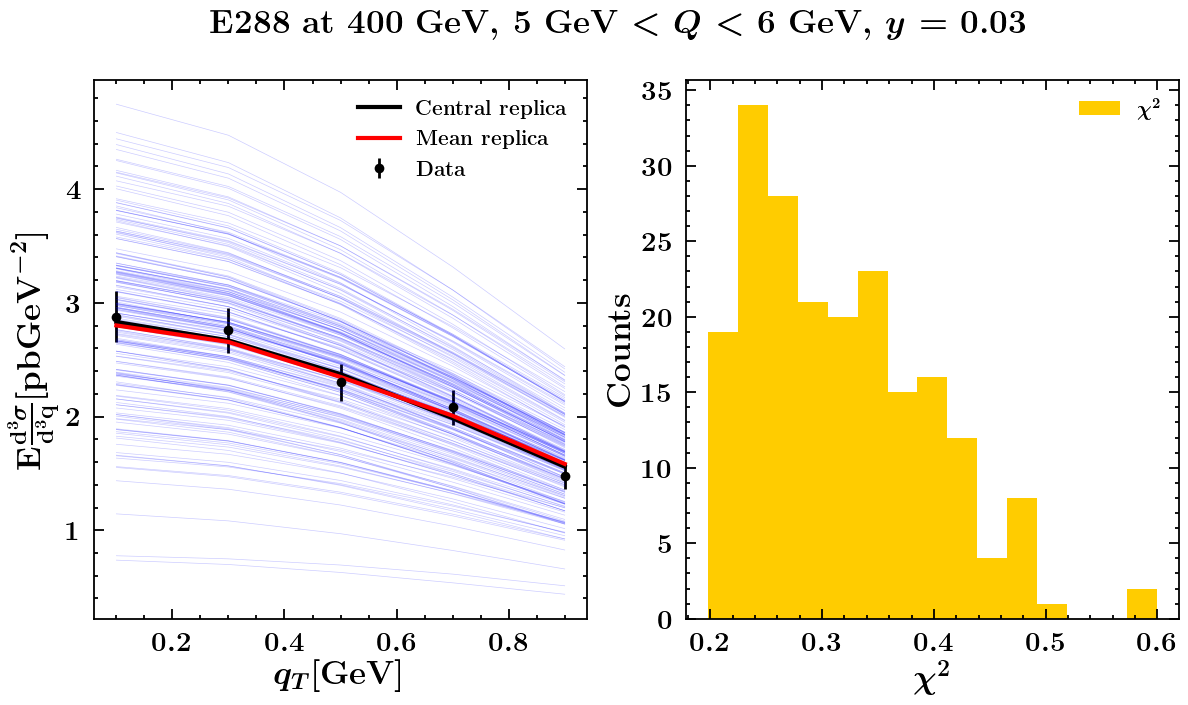
\includegraphics{pngplots/E288_400_Q_5_6.png}
\caption{E288\_400\_Q\_5\_6 data-theory comparison}
\end{figure}

\begin{figure}
\centering
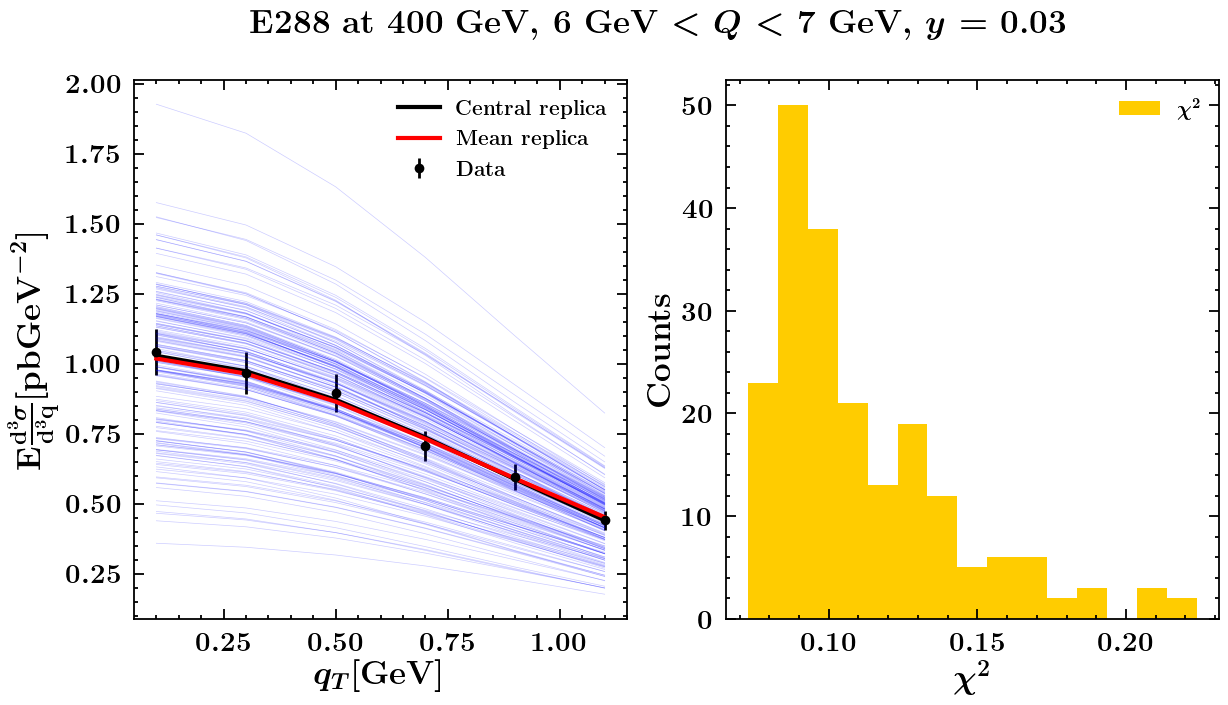
\includegraphics{pngplots/E288_400_Q_6_7.png}
\caption{E288\_400\_Q\_6\_7 data-theory comparison}
\end{figure}

\begin{figure}
\centering
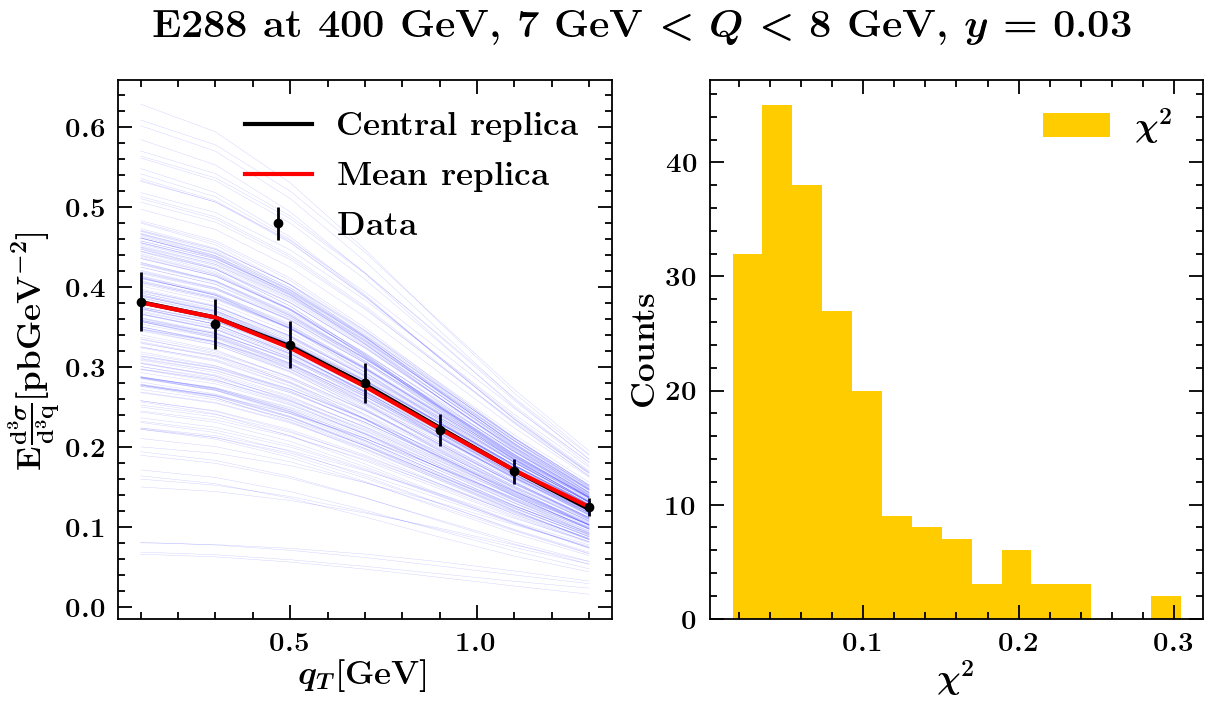
\includegraphics{pngplots/E288_400_Q_7_8.png}
\caption{E288\_400\_Q\_7\_8 data-theory comparison}
\end{figure}

\begin{figure}
\centering
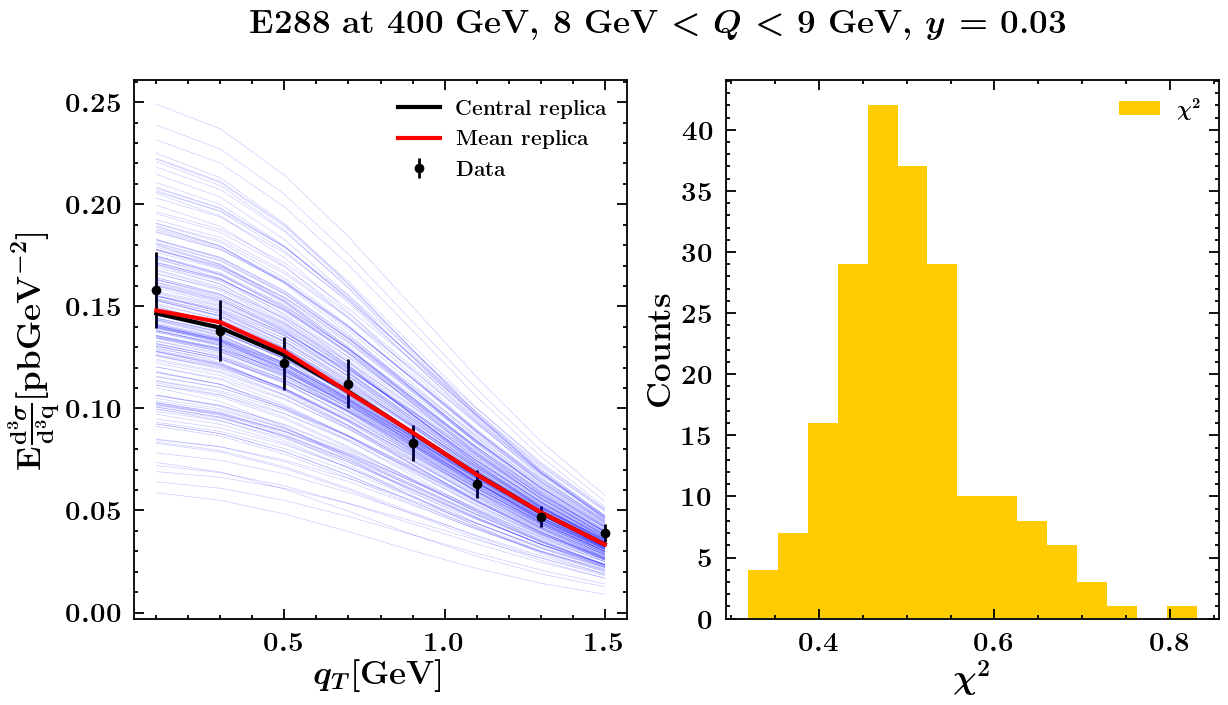
\includegraphics{pngplots/E288_400_Q_8_9.png}
\caption{E288\_400\_Q\_8\_9 data-theory comparison}
\end{figure}

\begin{figure}
\centering
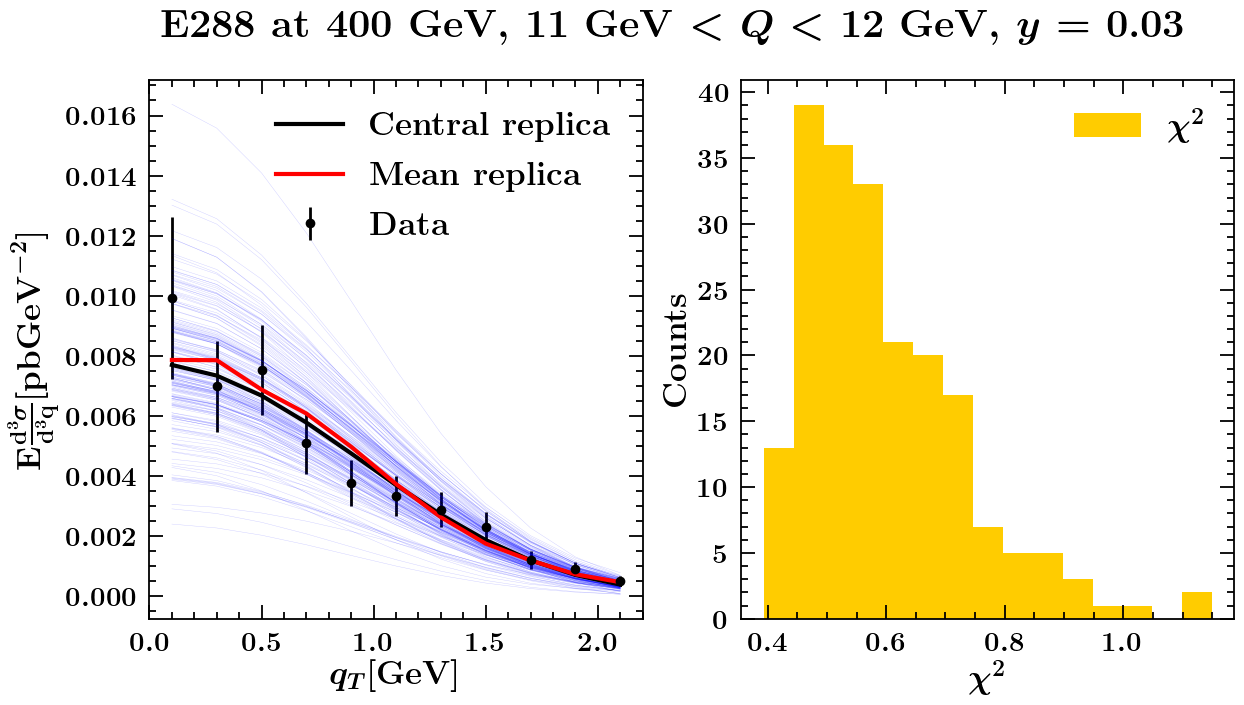
\includegraphics{pngplots/E288_400_Q_11_12.png}
\caption{E288\_400\_Q\_11\_12 data-theory comparison}
\end{figure}

\begin{figure}
\centering
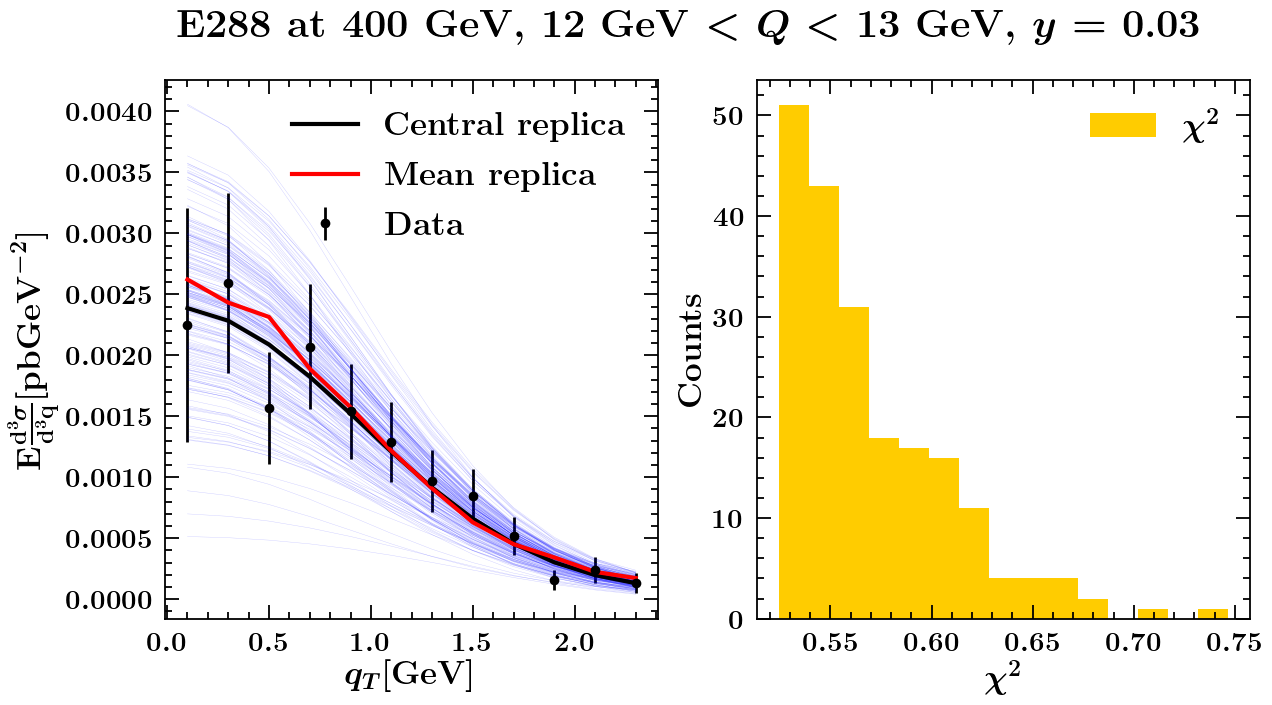
\includegraphics{pngplots/E288_400_Q_12_13.png}
\caption{E288\_400\_Q\_12\_13 data-theory comparison}
\end{figure}

\begin{figure}
\centering
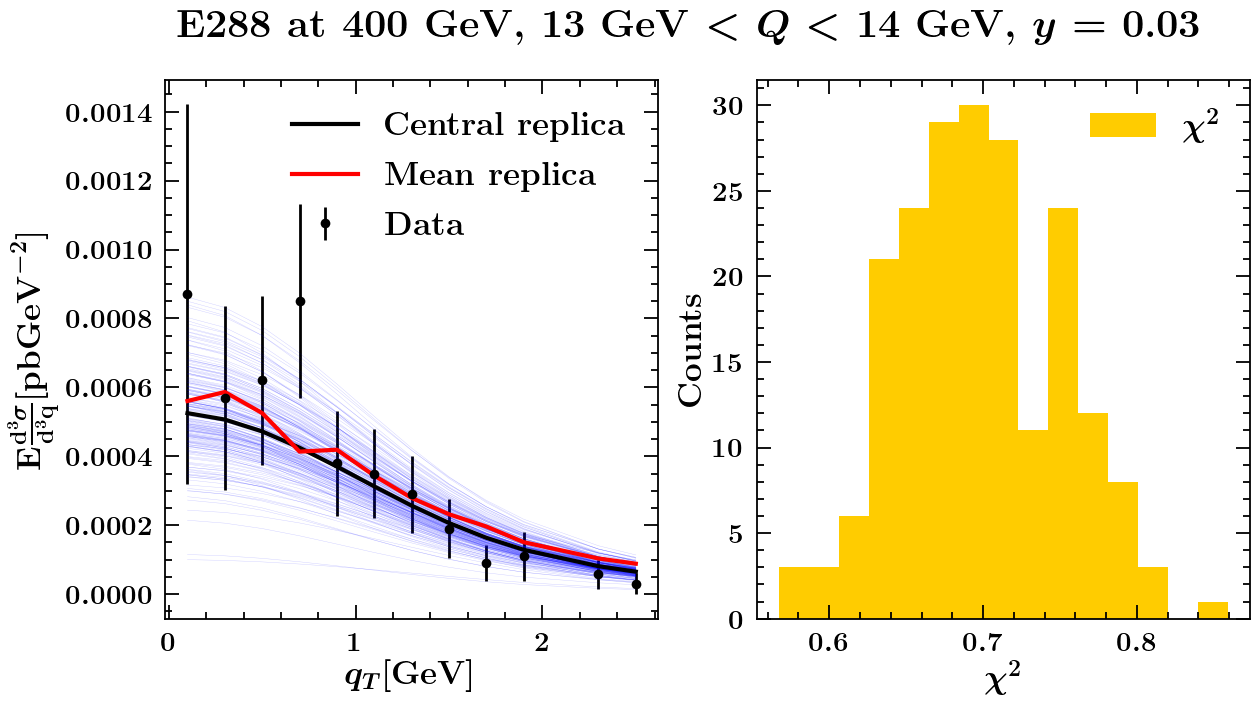
\includegraphics{pngplots/E288_400_Q_13_14.png}
\caption{E288\_400\_Q\_13\_14 data-theory comparison}
\end{figure}

\begin{figure}
\centering
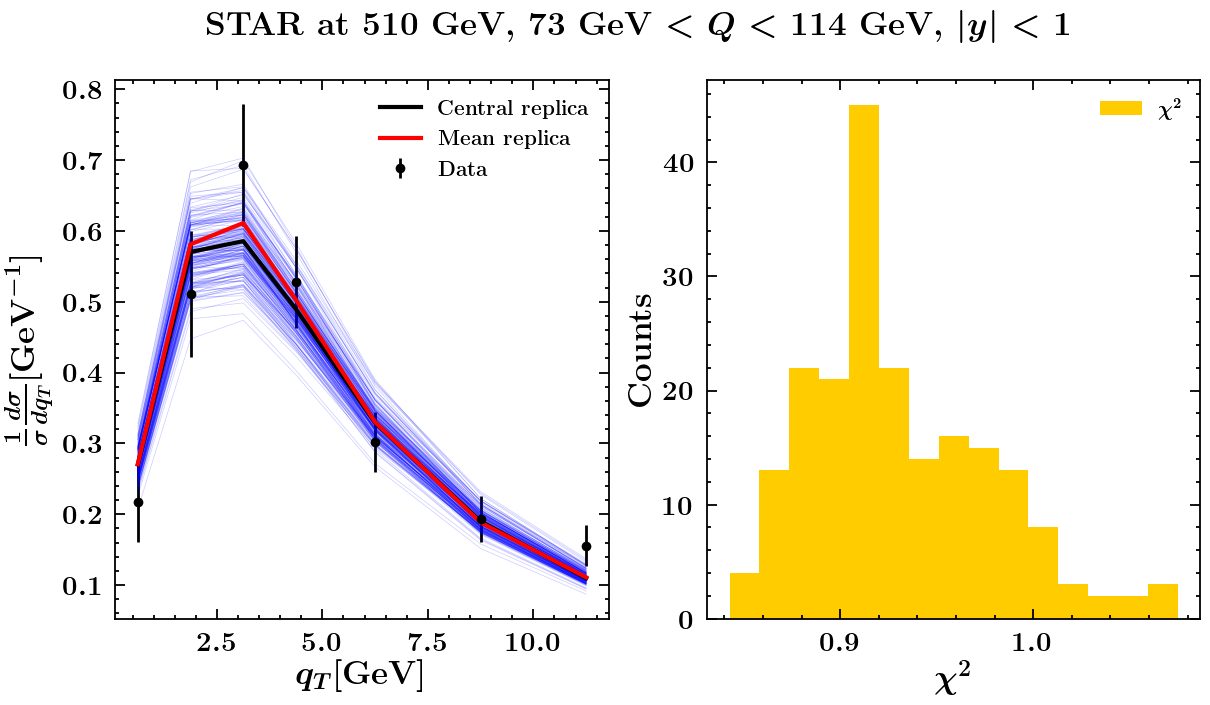
\includegraphics{pngplots/STAR_510.png}
\caption{STAR\_510 data-theory comparison}
\end{figure}

\begin{figure}
\centering
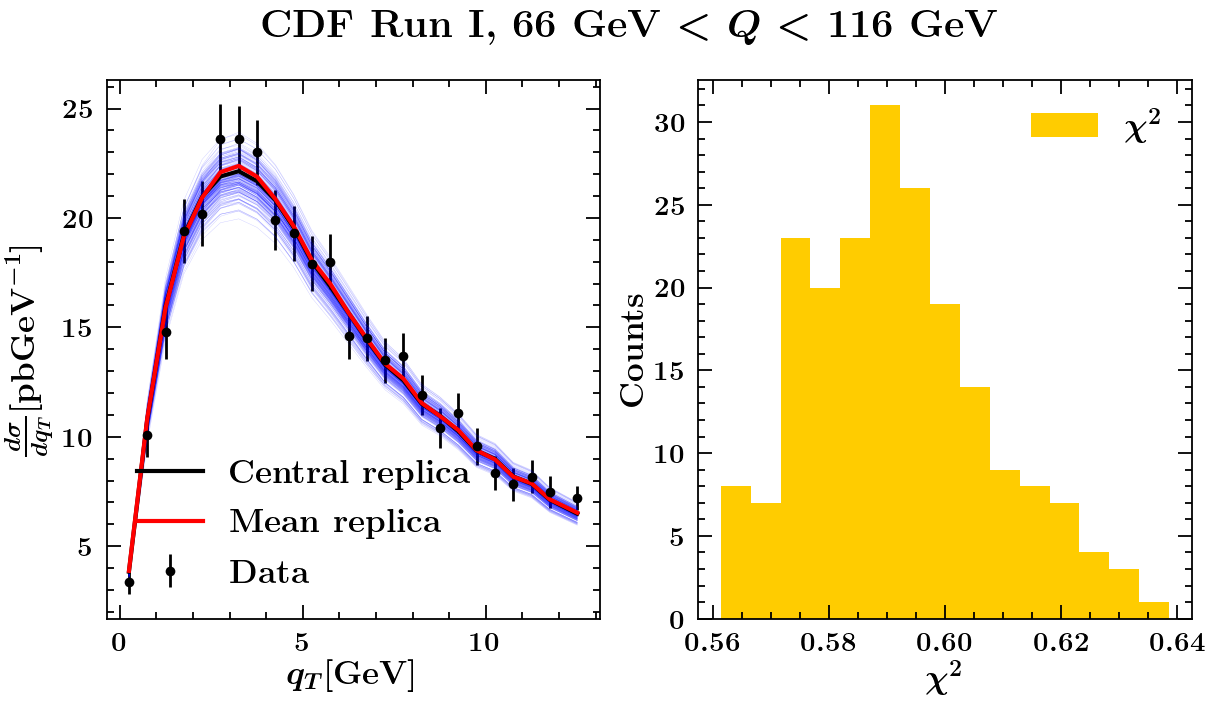
\includegraphics{pngplots/CDF_RunI.png}
\caption{CDF\_RunI data-theory comparison}
\end{figure}

\begin{figure}
\centering
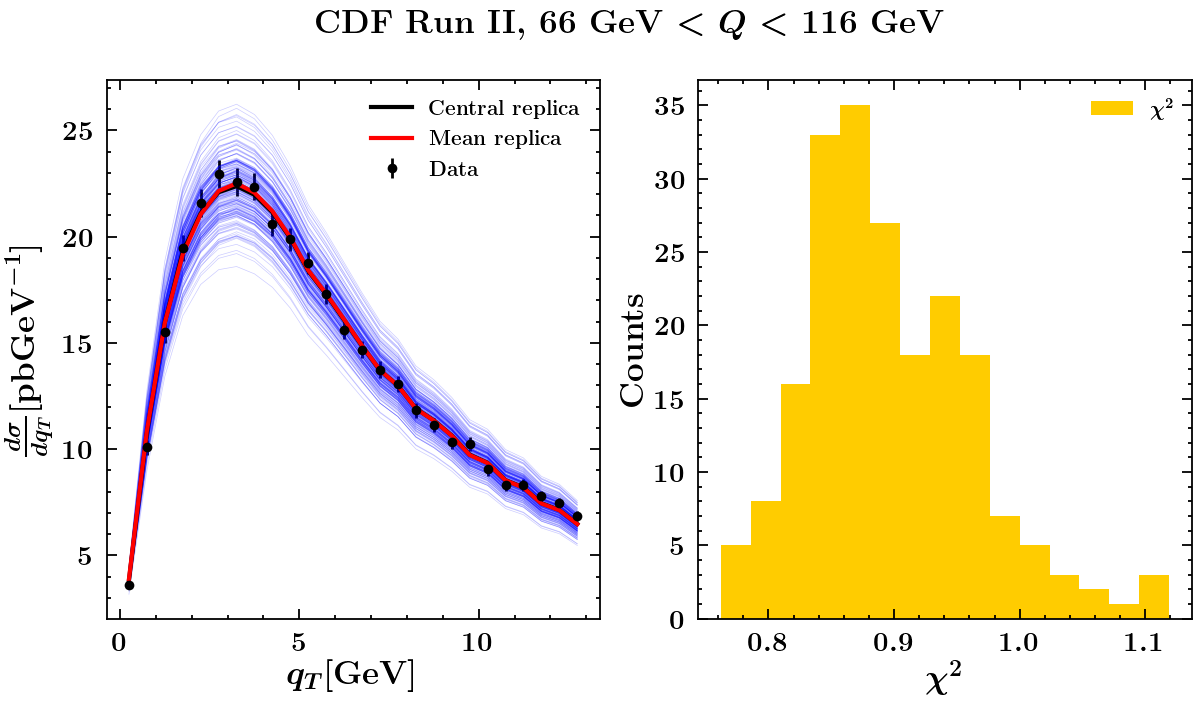
\includegraphics{pngplots/CDF_RunII.png}
\caption{CDF\_RunII data-theory comparison}
\end{figure}

\begin{figure}
\centering
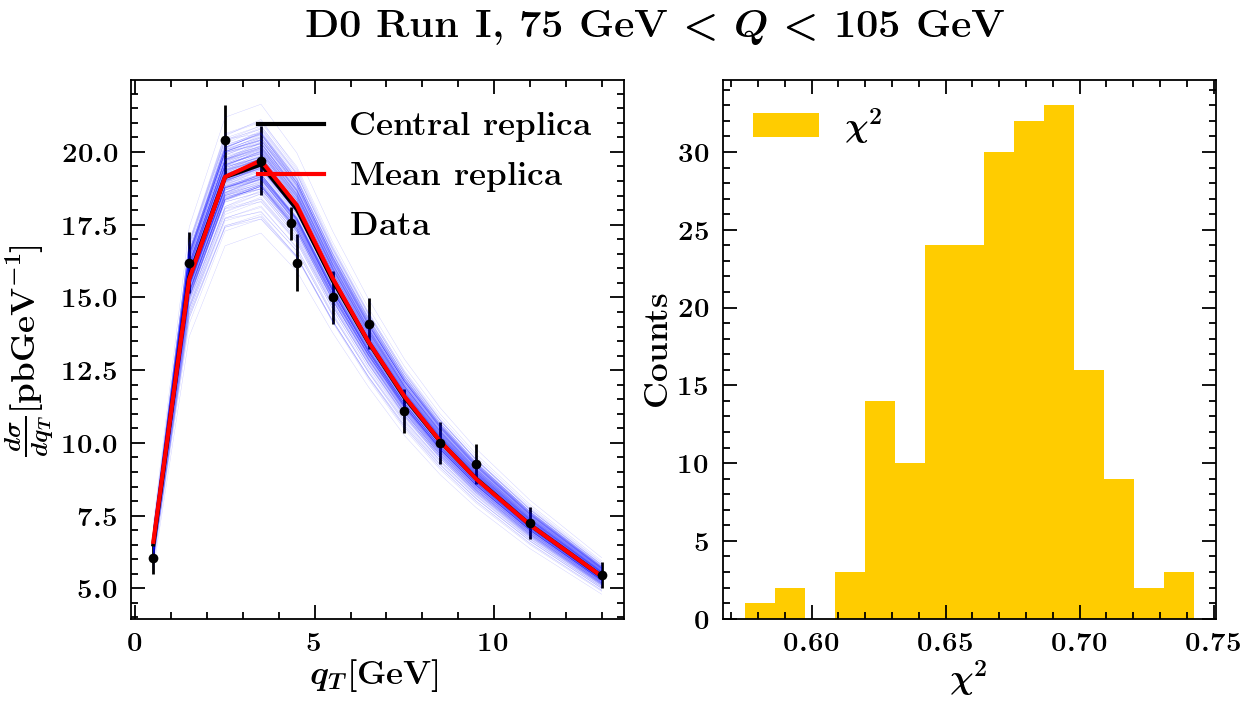
\includegraphics{pngplots/D0_RunI.png}
\caption{D0\_RunI data-theory comparison}
\end{figure}

\begin{figure}
\centering
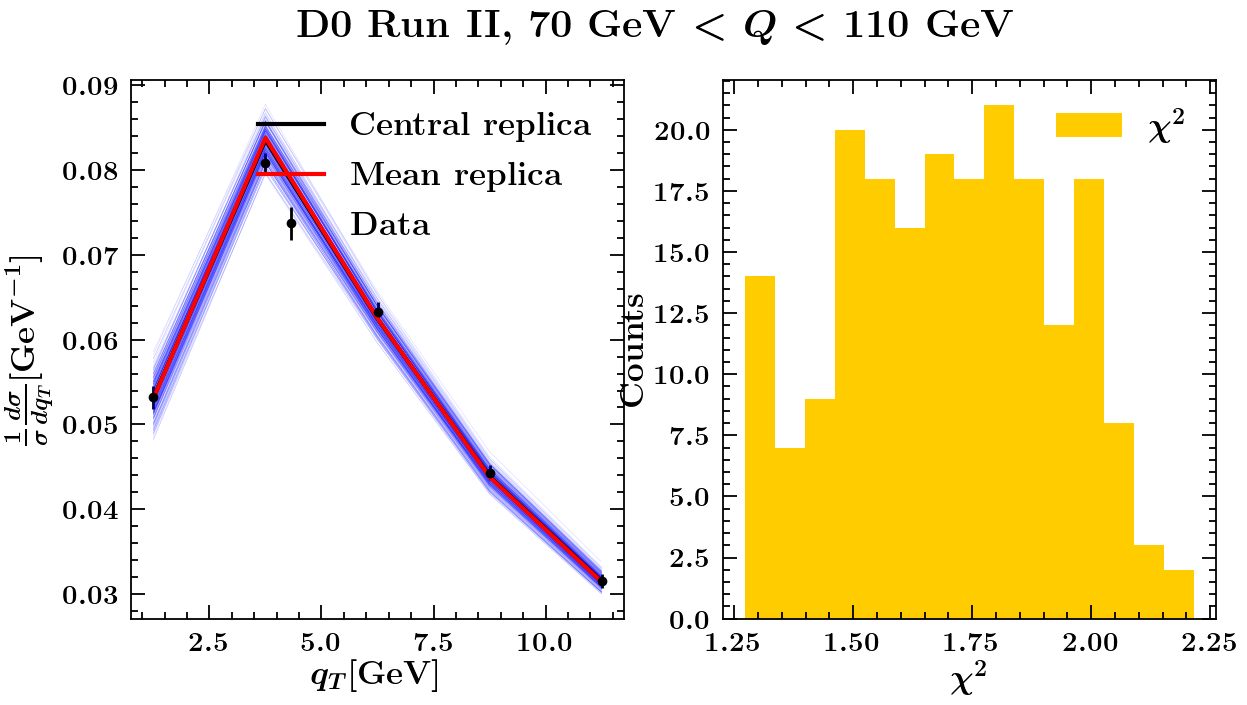
\includegraphics{pngplots/D0_RunII.png}
\caption{D0\_RunII data-theory comparison}
\end{figure}

\begin{figure}
\centering
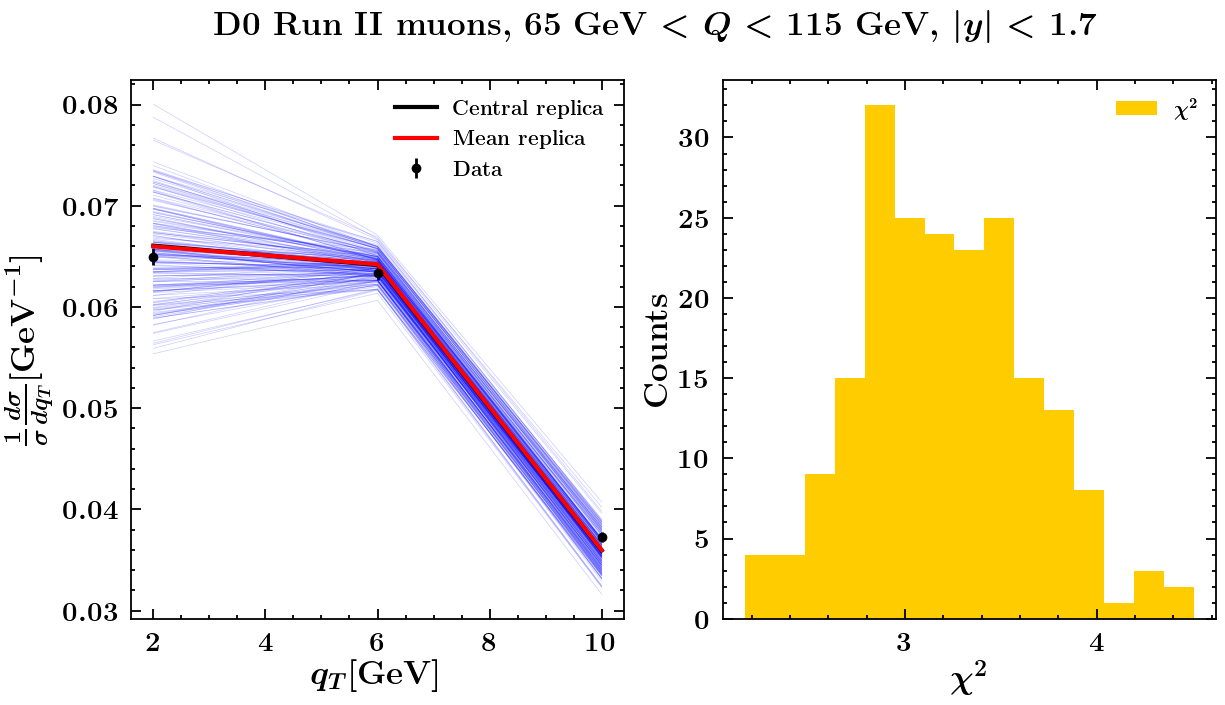
\includegraphics{pngplots/D0_RunIImu.png}
\caption{D0\_RunIImu data-theory comparison}
\end{figure}

\begin{figure}
\centering
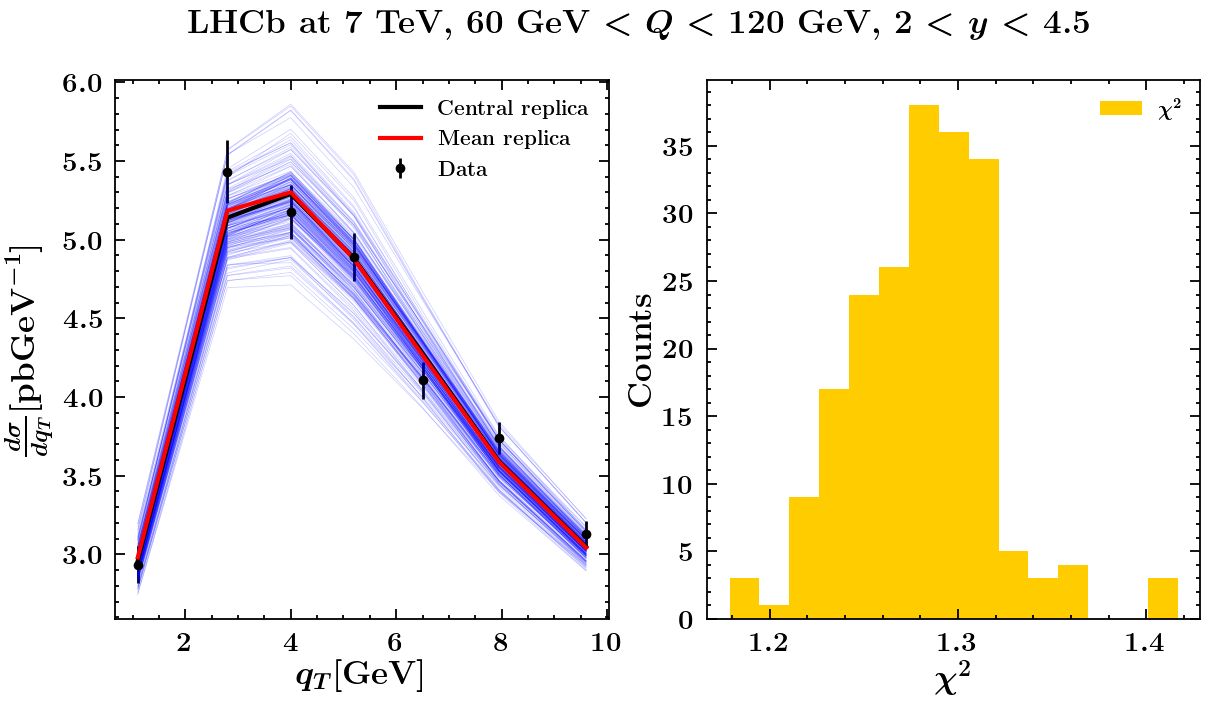
\includegraphics{pngplots/LHCb_7TeV.png}
\caption{LHCb\_7TeV data-theory comparison}
\end{figure}

\begin{figure}
\centering
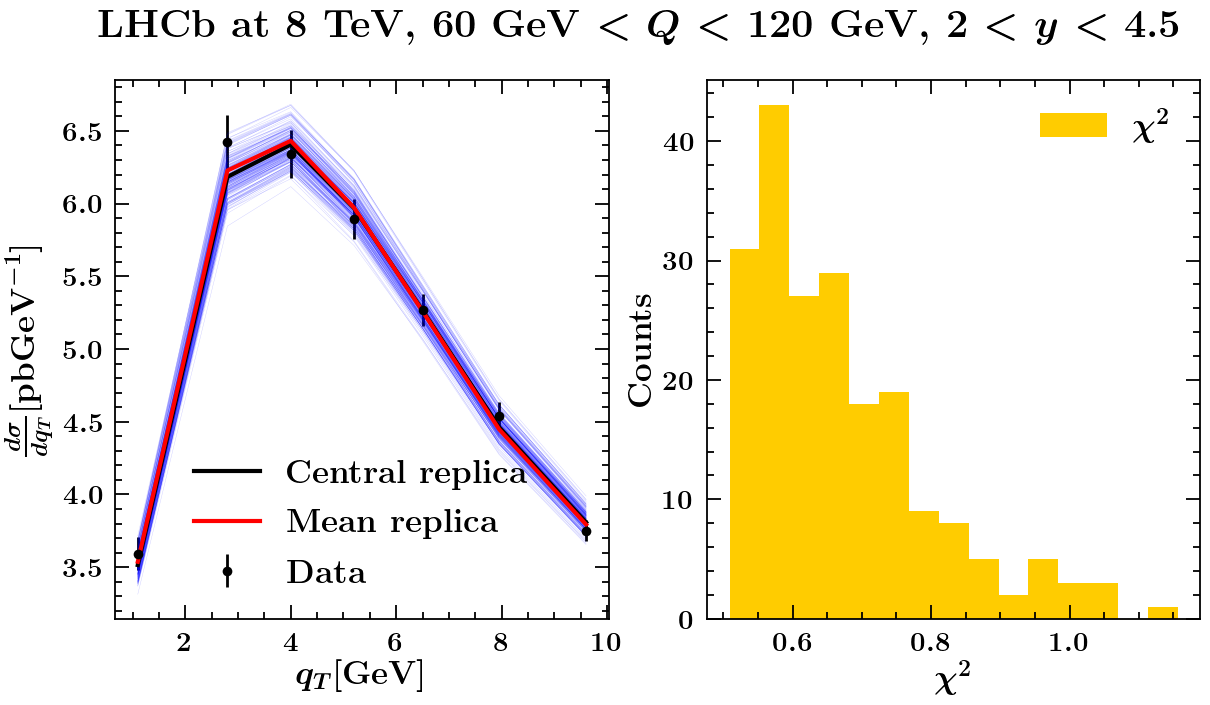
\includegraphics{pngplots/LHCb_8TeV.png}
\caption{LHCb\_8TeV data-theory comparison}
\end{figure}

\begin{figure}
\centering
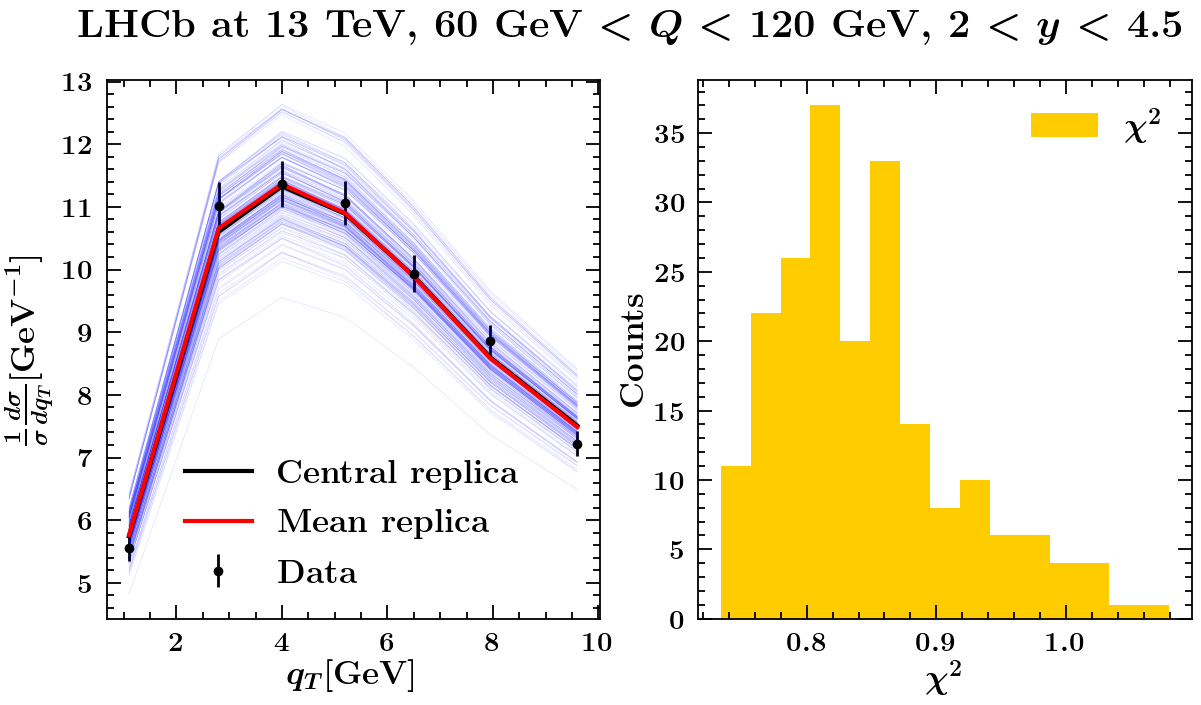
\includegraphics{pngplots/LHCb_13TeV.png}
\caption{LHCb\_13TeV data-theory comparison}
\end{figure}

\begin{figure}
\centering
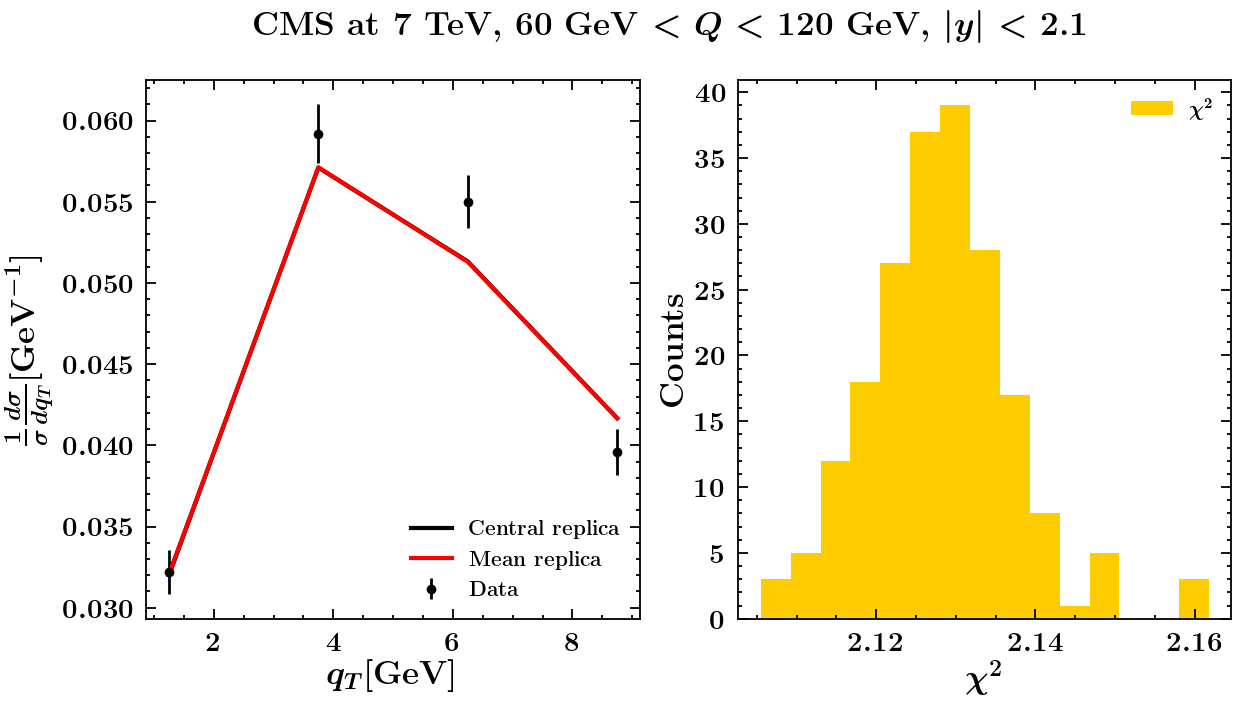
\includegraphics{pngplots/CMS_7TeV.png}
\caption{CMS\_7TeV data-theory comparison}
\end{figure}

\begin{figure}
\centering
\includegraphics{pngplots/CMS_8TeV.png}
\caption{CMS\_8TeV data-theory comparison}
\end{figure}

\begin{figure}
\centering
\includegraphics{pngplots/ATLAS_7TeV_y_0_1.png}
\caption{ATLAS\_7TeV\_y\_0\_1 data-theory comparison}
\end{figure}

\begin{figure}
\centering
\includegraphics{pngplots/ATLAS_7TeV_y_1_2.png}
\caption{ATLAS\_7TeV\_y\_1\_2 data-theory comparison}
\end{figure}

\begin{figure}
\centering
\includegraphics{pngplots/ATLAS_7TeV_y_2_2.4.png}
\caption{ATLAS\_7TeV\_y\_2\_2.4 data-theory comparison}
\end{figure}

\begin{figure}
\centering
\includegraphics{pngplots/ATLAS_8TeV_y_0_0.4.png}
\caption{ATLAS\_8TeV\_y\_0\_0.4 data-theory comparison}
\end{figure}

\begin{figure}
\centering
\includegraphics{pngplots/ATLAS_8TeV_y_0.4_0.8.png}
\caption{ATLAS\_8TeV\_y\_0.4\_0.8 data-theory comparison}
\end{figure}

\begin{figure}
\centering
\includegraphics{pngplots/ATLAS_8TeV_y_0.8_1.2.png}
\caption{ATLAS\_8TeV\_y\_0.8\_1.2 data-theory comparison}
\end{figure}

\begin{figure}
\centering
\includegraphics{pngplots/ATLAS_8TeV_y_1.2_1.6.png}
\caption{ATLAS\_8TeV\_y\_1.2\_1.6 data-theory comparison}
\end{figure}

\begin{figure}
\centering
\includegraphics{pngplots/ATLAS_8TeV_y_1.6_2.png}
\caption{ATLAS\_8TeV\_y\_1.6\_2 data-theory comparison}
\end{figure}

\begin{figure}
\centering
\includegraphics{pngplots/ATLAS_8TeV_y_2_2.4.png}
\caption{ATLAS\_8TeV\_y\_2\_2.4 data-theory comparison}
\end{figure}

\begin{figure}
\centering
\includegraphics{pngplots/ATLAS_8TeV_Q_46_66.png}
\caption{ATLAS\_8TeV\_Q\_46\_66 data-theory comparison}
\end{figure}

\begin{figure}
\centering
\includegraphics{pngplots/ATLAS_8TeV_Q_116_150.png}
\caption{ATLAS\_8TeV\_Q\_116\_150 data-theory comparison}
\end{figure}

\end{document}
